\begin{dang}{Bài toán thực tế}
Gắn hệ trục toạ độ vào mô hình. Đặt gốc toạ độ tại vị trí có "3 góc vuông"
% \newcommand{\gv}[4][black]{\draw[#1,thick] ($(#3)!8pt!(#2)$)--($(#3)!2!($($(#3)!8pt!(#2)$)!.5!($(#3)!8pt!(#4)$)$)$)--($(#3)!8pt!(#4)$);}
% \begin{longtable}{|>{\raggedright\arraybackslash}p{5.2cm}|>{\raggedright\arraybackslash}p{5.4cm}|>{\raggedright\arraybackslash}p{5.7cm}|}
% 		\hline
% 	    \multicolumn{3}{|>{\centering\arraybackslash}p{16.5cm}|}{\textbf{I. Gắn trục tọa độ đối với hình chóp}} \\ \hline    
% 	    \multicolumn{3}{|>{\centering\arraybackslash}p{16.5cm}|}{\textbf{1. Hình chóp có cạnh bên (SA) vuông góc với mặt đáy}} \\ \hline                                                                                                                                                                               
% 		\multicolumn{1}{|>{\raggedright\arraybackslash}p{5.2cm}|}{\begin{tabular}[l]{>{\raggedright\arraybackslash}p{5.2cm}} \textbf{Đáy là tam giác đều}
% 							\begin{tikzpicture}[>=stealth,font=\footnotesize]
% 							\def\a{3}
% 							\def\b{2}
% 							\def\h{2}
% 							\path (0:0) coordinate (A)
% 							++(0:\a) coordinate (C)
% 							++(-130:\b) coordinate (B)
% 							($(A)+(90:\h)$) coordinate (S)
% 							($(B)!1/2!(C)$) coordinate (O)
% 							($(O)+(90:3.5)$) coordinate (O1)
% 							($(S)+(O)-(A)$) coordinate (H);
% 							\draw[dashed,thick] (A)--(C);
% 							\draw[thick] (S)--(A)--(B)--(C)--(S)--(B);
% 							\draw[dashed,thick](A)--(O);
% 							\draw[thick](S)--(H);
% 							%Ve truc Ox,Oy, Oz
% 							\draw[thick,->](C)--($(O)!2!(C)$) node [pos=0.9,above ]{$x$};
% 							\draw[thick,->](A)--($(O)!1.2!(A)$) node [pos=0.9,above right]{$y$};
% 							\draw[thick,->](O)--(O1) node [pos=0.9,above right]{$z$};
% 							%Các góc vuông
% 							\gv{S}{H}{O}
% 							\gv{C}{O}{H}
% 							\gv{A}{O}{H}
% 							\gv{O}{A}{S}
% 							\foreach \x/\g in {A/-90,B/0,C/0,S/180,O/-10,H/-10}
% 							\fill[black] (\x) circle (1pt) ($(\g:4mm)+(\x)$) node {$\x$};	
% 						\end{tikzpicture}
				 
% 				 - Gọi $O$ là trung điểm $BC$. Chọn hệ trục tọa độ như hình vẽ, $AB=a=1$.
				
% 				- Tọa độ các điểm là:
						
% 						$O(0;0;0)$, $A \left(0;\dfrac{\sqrt{3}}{2};0\right)$, $B \left(\dfrac{-1}{2};0;0\right)$, $C \left(\dfrac{1}{2};0;0\right)$, $S \left(0;\dfrac{\sqrt{3}}{2};\underbrace {OH}_{ = SA}\right)$.
% 				\end{tabular}} &\multicolumn{1}{l|}{\begin{tabular}[l]{>{\raggedright\arraybackslash}p{5.2cm}}\textbf{Đáy là tam giác cân tại A}
				
% 					\begin{tikzpicture}[>=stealth,font=\footnotesize]
% 						\def\a{3.5}
% 						\def\b{2.5}
% 						\def\h{3.5}
% 						\path (0:0) coordinate (B)
% 						++(0:\a) coordinate (C)
% 						++(-150:\b) coordinate (A)
% 						($(B)!1/2!(C)$) coordinate (O)
% 						($(A)+(90:\h)$) coordinate (S)
% 						($(O)+(90:3.8)$) coordinate (O1)
% 						($(S)+(O)-(A)$) coordinate (H);
% 						\draw[dashed,thick] (B)--(C);
% 						\draw[thick] (S)--(B)--(A)--(C)--(S)--(A);
% 						\draw[dashed,thick](A)--(O);
% 						\draw[thick](S)--(H);
% 						%Ve truc Ox,Oy, Oz
% 						\draw[thick,->](C)--($(O)!1.4!(C)$) node [pos=0.9,below]{$x$};
% 						\draw[thick,->](A)--($(O)!1.4!(A)$) node [pos=0.9,below left]{$y$};
% 						\draw[thick,->](O)--(O1) node [pos=0.9,above right]{$z$};
% 						%Các góc vuông
% 						\gv{B}{A}{S}
% 						\gv{A}{O}{C}
% 						\foreach \x/\g in {A/-20,B/120,C/-50,S/180,O/40,H/180}
% 						\fill[black] (\x) circle (1pt) ($(\g:4mm)+(\x)$) node {$\x$};	
% 					\end{tikzpicture}
					
% 			- Gọi $O$ là trung điểm $BC$. Chọn hệ trục tọa độ như hình vẽ, $a=1$.
			
% 			- Tọa độ các điểm là:
				
% 				$O(0;0;0)$, $A \left(0;OA;0\right)$, $B \left(-OB;0;0\right)$, $C \left(OC;0;0\right)$, $S \left(0;OA;\underbrace {OH}_{ = SA}\right)$.
% 			\end{tabular}} & \begin{tabular}[l]{>{\raggedright\arraybackslash}p{5.6cm}}\textbf{ Đáy là tam giác cân tại B}
			
% 				\begin{tikzpicture}[>=stealth,font=\footnotesize]
% 					\def\a{3}
% 					\def\b{2}
% 					\def\h{2}
% 					\path (0:0) coordinate (A)
% 					++(0:\a) coordinate (C)
% 					++(-150:\b) coordinate (B)
% 					($(A)!1/2!(C)$) coordinate (O)
% 					($(A)+(90:\h)$) coordinate (S)
% 					($(O)+(90:2.5)$) coordinate (O1)
% 					($(S)+(O)-(A)$) coordinate (H);
% 					\draw[dashed,thick] (A)--(C);
% 					\draw[thick] (S)--(A)--(B)--(C)--(S)--(B);
% 					\draw[dashed,thick](B)--(O) ;
% 					\draw[thick](S)--(H);
% 					%Ve truc Ox,Oy, Oz
% 					\draw[thick,->](C)--($(O)!1.4!(C)$) node [pos=0.9,below]{$x$};
% 					\draw[thick,->](B)--($(O)!1.2!(B)$) node [pos=0.9,below left]{$y$};
% 					\draw[dashed,thick](O)--($(O)!1/2!(H)$);
% 					\draw[thick,->]($(O)!1/2!(H)$)--(O1) node [pos=0.9,above right]{$z$};
% 					%Các góc vuông
% 					\gv{S}{A}{C}
% 					\gv{B}{O}{C}
% 					\foreach \x/\g in {B/-20,A/120,C/-50,S/180,O/40,H/-10}
% 					\fill[black] (\x) circle (1pt) ($(\g:4mm)+(\x)$) node {$\x$};	
% 				\end{tikzpicture}
				
% 			- Gọi $O$ là trung điểm $BC$. Chọn hệ trục tọa độ như hình vẽ, $AB=a=1$.
			
% 			- Tọa độ các điểm là:
			
% 			$O(0;0;0)$, $A \left(\dfrac{-1}{2};0;0\right)$, $B \left(0;\dfrac{\sqrt{3}}{2};0\right)$, $C \left(\dfrac{1}{2};0;0\right)$, $S \left(0;\dfrac{\sqrt{3}}{2};\underbrace {OH}_{ = SA}\right)$.
% 	\end{tabular} \\ \hline
% 	\multicolumn{1}{|>{\raggedright\arraybackslash}p{5.2cm}|}{\begin{tabular}[l]{>{\raggedright\arraybackslash}p{5.2cm}} \textbf{Đáy là tam giác vuông tại $B$}
			
% 			\begin{tikzpicture}[>=stealth,font=\footnotesize,scale=1]
% 				\def\a{4}
% 				\def\b{3}
% 				\def\h{2.6}
% 				\path (0:0) coordinate (A)
% 				++(0:\a) coordinate (C)
% 				++(-150:\b) coordinate (B)
% 				($(C)!1.01!(B)$) coordinate (O)
% 				($(A)+(90:\h)$) coordinate (S)
% 				($(O)+(90:3.5)$) coordinate (O1)
% 				($(S)+(O)-(A)$) coordinate (H);
% 				\draw[dashed,thick] (A)--(C);
% 				\draw[thick] (S)--(A)--(B)--(C)--(S)--(B);
% 				\draw[thick](S)--(H);
% 				%Ve truc Ox,Oy, Oz
% 				\draw[thick,->](C)--($(O)!1.1!(C)$) node [pos=0.9,above ]{$x$};
% 				\draw[thick,->](A)--($(O)!1.2!(A)$) node [pos=0.9, above]{$y$};
% 				\draw[thick,->](O)--(O1) node [above]{$z$};
% 				%Các góc vuông
% 				\gv{H}{O}{A}
% 				\gv{C}{B}{A}
% 				\gv{C}{A}{S}
% 				\gv{S}{H}{B}
% 				\foreach \x/\g in {A/-90,B/0,C/-40,S/90,O/-110,H/-10}
% 				\fill[black] (\x) circle (1pt) ($(\g:4mm)+(\x)$) node {$\x$};	
% 			\end{tikzpicture}
% 	\end{tabular}} &\multicolumn{1}{l|}{\begin{tabular}[l]{>{\raggedright\arraybackslash}p{5.2cm}}\textbf{Đáy là tam giác vuông tại $A$}
	
% 	\begin{tikzpicture}[>=stealth,font=\footnotesize,scale=1]
% 		\def\a{3.5}
% 		\def\b{4}
% 		\def\h{3}
% 		\path (0:0) coordinate (O)
% 		++(0:\a) coordinate (C)
% 		++(-165:\b) coordinate (B)
% 		($(A)+(90:\h)$) coordinate (S)
% 		($(O)+(90:3.3)$) coordinate (O1)
% 		($(C)!1!(O)$) coordinate (A);
% 		\draw[dashed,thick] (B)--(A)--(C) (O)--(S);
% 		\draw[thick] (S)--(B)--(C)--(S);
% 		%Ve truc Ox,Oy, Oz
% 		\draw[thick,->](C)--($(O)!1.2!(C)$) node [pos=0.9,below]{$x$};
% 		\draw[thick,->](B)--($(O)!1.25!(B)$) node [pos=0.9,right]{$y$};
% 		\draw[thick,->](S)--(O1) node [pos=0.9,above right]{$z$};
% 		%Các góc vuông
% 		\gv{B}{O}{C}
% 		\gv{A}{O}{C}
% 		\foreach \x/\g in {A/-45,B/120,C/-50,S/180,O/145}
% 		\fill[black] (\x) circle (1pt) ($(\g:4mm)+(\x)$) node {$\x$};	
% 	\end{tikzpicture}
% 	\end{tabular}} & \begin{tabular}[l]{>{\raggedright\arraybackslash}p{5.6cm}}\textbf{Đáy là tam giác thường}
% 	\begin{tikzpicture}[>=stealth,font=\footnotesize,scale=1]
% 	\def\a{3.8}
% 	\def\b{3}
% 	\def\h{2}
% 	\path (0:0) coordinate (A)
% 	++(0:\a) coordinate (C)
% 	++(-150:\b) coordinate (B)
% 	($(A)!1/2!(C)$) coordinate (O)
% 	($(A)+(90:\h)$) coordinate (S)
% 	($(O)+(90:2.5)$) coordinate (O1)
% 	($(S)+(O)-(A)$) coordinate (H);
% 	\draw[dashed,thick] (A)--(C);
% 	\draw[thick] (S)--(A)--(B)--(C)--(S)--(B);
% 	\draw[dashed,thick](B)--(O) ;
% 	\draw[thick](S)--(H);
% 	%Ve truc Ox,Oy, Oz
% 	\draw[thick,->](C)--($(O)!1.4!(C)$) node [pos=0.9,below]{$x$};
% 	\draw[thick,->](B)--($(O)!1.2!(B)$) node [pos=0.9,below left]{$y$};
% 	\draw[dashed,thick](O)--($(O)!1/2!(H)$);
% 	\draw[thick,->]($(O)!1/2!(H)$)--(O1) node [pos=0.9,above right]{$z$};
% 	%Các góc vuông
% 	\gv{S}{A}{C}
% 	\gv{B}{O}{C}
% 	\foreach \x/\g in {B/-20,A/120,C/-50,S/180,O/40,H/-10}
% 	\fill[black] (\x) circle (1pt) ($(\g:4mm)+(\x)$) node {$\x$};	
% 	\end{tikzpicture}
% 	\end{tabular} \\ \hline
% 	\end{longtable}
% \begin{longtable}{|>{\raggedright\arraybackslash}p{5.4cm}|>{\raggedright\arraybackslash}p{5.2cm}|>{\raggedright\arraybackslash}p{5.8cm}|}
% 	\hline
% 	{\begin{tabular}[l]{>{\raggedright\arraybackslash}p{4.8cm}} \textbf{Đáy là tam giác vuông tại $B$}
			
% 			\begin{tikzpicture}[>=stealth,font=\footnotesize,scale=1]
% 				\def\a{4}
% 				\def\b{3}
% 				\def\h{2.6}
% 				\path (0:0) coordinate (A)
% 				++(0:\a) coordinate (C)
% 				++(-150:\b) coordinate (B)
% 				($(C)!1.01!(B)$) coordinate (O)
% 				($(A)+(90:\h)$) coordinate (S)
% 				($(O)+(90:3.5)$) coordinate (O1)
% 				($(S)+(O)-(A)$) coordinate (H);
% 				\draw[dashed,thick] (A)--(C);
% 				\draw[thick] (S)--(A)--(B)--(C)--(S)--(B);
% 				\draw[thick](S)--(H);
% 				%Ve truc Ox,Oy, Oz
% 				\draw[thick,->](C)--($(O)!1.1!(C)$) node [pos=0.9,above ]{$x$};
% 				\draw[thick,->](A)--($(O)!1.2!(A)$) node [pos=0.9, above]{$y$};
% 				\draw[thick,->](O)--(O1) node [above]{$z$};
% 				%Các góc vuông
% 				\gv{H}{O}{A}
% 				\gv{C}{B}{A}
% 				\gv{C}{A}{S}
% 				\gv{S}{H}{B}
% 				\foreach \x/\g in {A/-90,B/0,C/-40,S/90,O/-110,H/-10}
% 				\fill[black] (\x) circle (1pt) ($(\g:4mm)+(\x)$) node {$\x$};	
% 			\end{tikzpicture}
		
% 			- Chọn hệ trục tọa độ như hình vẽ, $a=1$.
			
% 			- Tọa độ các điểm là:
				
% 				$B \equiv O(0;0;0)$, $A \left(0;AB;0\right)$, $C \left(BC;0;0\right)$, $S \left(0;AB;\underbrace {BH}_{ = SA}\right)$.
	
% 	\end{tabular}}&{\begin{tabular}[l]{>{\raggedright\arraybackslash}p{5cm}}\textbf{Đáy là tam giác vuông tại $A$}
			
% 			\begin{tikzpicture}[>=stealth,font=\footnotesize,scale=1]
% 				\def\a{3.5}
% 				\def\b{4}
% 				\def\h{3}
% 				\path (0:0) coordinate (O)
% 				++(0:\a) coordinate (C)
% 				++(-165:\b) coordinate (B)
% 				($(A)+(90:\h)$) coordinate (S)
% 				($(O)+(90:3.3)$) coordinate (O1)
% 				($(C)!1!(O)$) coordinate (A);
% 				\draw[dashed,thick] (B)--(A)--(C) (O)--(S);
% 				\draw[thick] (S)--(B)--(C)--(S);
% 				%Ve truc Ox,Oy, Oz
% 				\draw[thick,->](C)--($(O)!1.2!(C)$) node [pos=0.9,below]{$x$};
% 				\draw[thick,->](B)--($(O)!1.25!(B)$) node [pos=0.9,right]{$y$};
% 				\draw[thick,->](S)--(O1) node [pos=0.9,above right]{$z$};
% 				%Các góc vuông
% 				\gv{B}{O}{C}
% 				\gv{A}{O}{C}
% 				\foreach \x/\g in {A/-45,B/120,C/-50,S/180,O/145}
% 				\fill[black] (\x) circle (1pt) ($(\g:4mm)+(\x)$) node {$\x$};	
% 			\end{tikzpicture}

% 			- Chọn hệ trục tọa độ như hình vẽ, $a=1$.
			
% 			- Tọa độ các điểm là:
				
% 				$A \equiv O(0;0;0)$, $B \left(0;OB;0\right)$, $C \left(AC;0;0\right)$, $S \left(0;0;SA \right)$.
	
% 	\end{tabular}}&{\begin{tabular}[l]{>{\raggedright\arraybackslash}p{5cm}} \textbf{Đáy là tam giác thường}
% 			\begin{tikzpicture}[>=stealth,font=\footnotesize,scale=1]
% 				\def\a{3.8}
% 				\def\b{3}
% 				\def\h{2}
% 				\path (0:0) coordinate (A)
% 				++(0:\a) coordinate (C)
% 				++(-150:\b) coordinate (B)
% 				($(A)!1/2!(C)$) coordinate (O)
% 				($(A)+(90:\h)$) coordinate (S)
% 				($(O)+(90:2.5)$) coordinate (O1)
% 				($(S)+(O)-(A)$) coordinate (H);
% 				\draw[dashed,thick] (A)--(C);
% 				\draw[thick] (S)--(A)--(B)--(C)--(S)--(B);
% 				\draw[dashed,thick](B)--(O) ;
% 				\draw[thick](S)--(H);
% 				%Ve truc Ox,Oy, Oz
% 				\draw[thick,->](C)--($(O)!1.4!(C)$) node [pos=0.9,below]{$x$};
% 				\draw[thick,->](B)--($(O)!1.2!(B)$) node [pos=0.9,below left]{$y$};
% 				\draw[dashed,thick](O)--($(O)!1/2!(H)$);
% 				\draw[thick,->]($(O)!1/2!(H)$)--(O1) node [pos=0.9,above right]{$z$};
% 				%Các góc vuông
% 				\gv{S}{A}{C}
% 				\gv{B}{O}{C}
% 				\foreach \x/\g in {B/-20,A/120,C/-50,S/180,O/40,H/-10}
% 				\fill[black] (\x) circle (1pt) ($(\g:4mm)+(\x)$) node {$\x$};	
% 			\end{tikzpicture}
			
% 				- Dựng đường cao $BO$ của $\triangle ABC$. Chọn hệ trục tọa độ như hình vẽ, $a=1$.\\
% 				- Tọa độ các điểm là:
			
% 				$O(0;0;0)$, $A \left(-OA;0;0\right)$, $B \left(0;OB;0\right)$, $C \left(OC;0;0\right)$, $S \left(-OA;0;\underbrace {OH}_{ = SA}\right)$.
% 	\end{tabular}}\\ \hline
% 	{\begin{tabular}[l]{>{\raggedright\arraybackslash}p{5cm}} \textbf{Đáy là hình vuông, hình chữ nhật}
			
% 			\begin{tikzpicture}[>=stealth,font=\footnotesize,scale=1]
% 				\def\a{3}
% 				\def\b{2}
% 				\def\h{2}
% 				\path 	(0:0) coordinate (A)
% 				++(0:\a) coordinate (D)
% 				++(-130:\b) coordinate (C)
% 				($(A)+(C)-(D)$) coordinate (B)
% 				($(A)+(90:\h)$) coordinate (S);
% 				\draw[dashed,thick] (S)--(A)--(B) (D)--(A);
% 				\draw[thick] (S)--(B)--(C)--(D)--(S)--(C);
% 				%Ve truc Ox,Oy, Oz
% 				\draw[thick,->](D)--($(A)!1.2!(D)$) node [pos=0.9,above ]{$x$};
% 				\draw[thick,->](B)--($(A)!1.2!(B)$) node [pos=0.9, above]{$y$};
% 				\draw[thick,->](S)--($(A)!1.2!(S)$) node [pos=0.9,above ]{$z$};
% 				%Các góc vuông
% 				\gv{D}{A}{S}
% 				\gv{D}{A}{B}
% 				\foreach \x/\g in {A/-90,B/-40,C/-40,D/-90,S/180}
% 				\fill[black] (\x) circle (1pt) ($(\g:4mm)+(\x)$) node {$\x$};	
% 			\end{tikzpicture}
		
% 			- Chọn hệ trục tọa độ như hình vẽ, $a=1$.
			
% 			- Tọa độ các điểm là:
			
% 			$A \equiv O(0;0;0)$, $B \left(0;AB;0\right)$, $C \left(AD;AB;0\right)$, $D(AD;0;0)$, $S \left(0;0;SA\right)$.
% \end{tabular}}&{\begin{tabular}[l]{>{\raggedright\arraybackslash}p{5cm}}\textbf{Đáy là hình thoi}
		
% 		\begin{tikzpicture}[>=stealth,font=\footnotesize,scale=1]
% 			\def\a{3}
% 			\def\b{2}
% 			\def\h{2}
% 			\path 	(0:0) coordinate (A)
% 			++(0:\a) coordinate (D)
% 			++(-130:\b) coordinate (C)
% 			($(A)+(C)-(D)$) coordinate (B)
% 			($(A)+(90:\h)$) coordinate (S)
% 			($(A)!1/2!(C)$) coordinate (O)
% 			($(S)+(O)-(A)$) coordinate (H);
% 			\draw[dashed,thick] (S)--(A)--(B) (D)--(A);
% 			\draw[thick] (S)--(B)--(C)--(D)--(S)--(C) (S)--(H);
% 			\draw[dashed,thick] (A)--(C) (B)--(D);
% 			%Ve truc Ox,Oy, Oz
% 			\draw[thick,->](A)--($(A)!-1/5!(C)$) node [pos=0.9,above ]{$x$};
% 			\draw[thick,->](B)--($(B)!-1/10!(D)$) node [pos=0.9, above]{$y$};
% 			\draw[thick,dashed](O)--($(O)!1/2!(H)$);
% 			\draw[thick,->]($(O)!1/2!(H)$)--($(O)!3/2!(H)$) node [pos=0.9,right ]{$z$};
	
% 			%Các góc vuông
% 			\gv{D}{A}{S}
% 			\gv{S}{H}{O}
% 			\gv{A}{O}{D}
% 			\foreach \x/\g in {A/-90,B/-40,C/-40,D/-90,S/180,O/-90,H/-40}
% 			\fill[black] (\x) circle (1pt) ($(\g:4mm)+(\x)$) node {$\x$};	
% 		\end{tikzpicture}
	
% 			- Chọn hệ trục tọa độ như hình vẽ, $a=1$.
			
% 			- Tọa độ các điểm là:
			
% 			$O(0;0;0)$, $A(OA;0;0)$, $B \left(0;OB;0\right)$, $C \left(-OC;0;0\right)$, $D(0;-OD;0)$, $S \left(OA;0;\underbrace {OH}_{ = SA} \right)$.
		
% \end{tabular}}&{\begin{tabular}[l]{>{\raggedright\arraybackslash}p{5.8cm}} \textbf{Đáy là hình thang vuông}
% 	\begin{tikzpicture}[>=stealth,font=\footnotesize,scale=1]
% 		\def\a{3}
% 		\def\b{2.1}
% 		\def\h{2.2}
% 		\path 	(0:0) coordinate (A)
% 		++(0:\a) coordinate (D)
% 		($(A)+(-140:\b)$) coordinate (B)
% 		($(A)+(90:\h)$) coordinate (S)
% 		($(A)!0.78!(D)$) coordinate (H)
% 		($(H)+(B)-(A)$) coordinate (C);
% 		\draw[dashed,thick] (S)--(A)--(B) (D)--(A) (C)--(H);
% 		\draw[thick] (S)--(B)--(C)--(D)--(S)--(C);
% 		%Ve truc Ox,Oy, Oz
% 		\draw[thick,->](D)--($(A)!1.2!(D)$) node [pos=0.9,above ]{$x$};
% 		\draw[thick,->](B)--($(A)!1.2!(B)$) node [pos=0.9, above]{$y$};
% 		\draw[thick,->](S)--($(A)!1.2!(S)$) node [pos=0.9,above ]{$z$};
% 		%Các góc vuông
% 		\gv{D}{A}{S}
% 		\gv{D}{A}{B}
% 		\gv{C}{H}{A}
% 		\foreach \x/\g in {A/-90,B/-40,C/-40,D/-90,S/180,H/120}
% 		\fill[black] (\x) circle (1pt) ($(\g:4mm)+(\x)$) node {$\x$};	
% 	\end{tikzpicture}
	
% 	 	- Chọn hệ trục tọa độ như hình vẽ, $a=1$.
	 
% 	 - Tọa độ các điểm là:
	 
% 	 $A \equiv O(0;0;0)$, $B \left(0;AB;0\right)$, $C \left(AH;AB;0\right)$, $D(AD;0;0)$, $S \left(0;0;SA\right)$.
% \end{tabular}}\\ \hline
% \end{longtable}
% \newpage
% 	\begin{longtable}{|>{\raggedright\arraybackslash}p{5cm}|>{\raggedright\arraybackslash}p{5cm}|>{\raggedright\arraybackslash}p{5cm}|}
% 	\hline
% 	\multicolumn{3}{|>{\centering\arraybackslash}p{16.5cm}|}{\textbf{2. Hình chóp có cạnh mặt bên $(SAB)$ vuông góc với mặt đáy}}                                                                                                                                                                                 \\ \hline
% 	\multicolumn{1}{|>{\raggedright\arraybackslash}p{5cm}|}{\begin{tabular}[l]{>{\raggedright\arraybackslash}p{4.5cm}} \textbf{Đáy là tam giác, mặt bên là tam giác thường}
% 			\begin{tikzpicture}[>=stealth,font=\footnotesize,scale=1]
% 				\def\a{4}
% 				\def\b{3}
% 				\def\h{3}
% 				\path (0:0) coordinate (A)
% 				++(0:\a) coordinate (C)
% 				++(-140:\b) coordinate (B)
% 				($(A)!0.55!(B)$) coordinate (O)
% 				($(A)!1/3!(B)$) coordinate (H)
% 				($(O)+(90:3.7)$) coordinate (O1)
% 				($(H)+(90:\h)$) coordinate (S)
% 				($(S)+(O)-(H)$) coordinate (K);
% 				\draw[dashed,thick] (A)--(C) (C)--(O);
% 				\draw[thick] (S)--(A)--(B)--(C)--(S)--(B);
% 				\draw[thick](S)--(H) (S)--(K);
% 				%Ve truc Ox,Oy, Oz
% 				\draw[thick,->](C)--($(O)!1.1!(C)$) node [pos=0.9,above ]{$x$};
% 				\draw[thick,->](A)--($(O)!1.3!(A)$) node [pos=0.9, above]{$y$};
% 				\draw[thick,->](O)--(O1) node [above]{$z$};
% 				%Các góc vuông
% 				\gv{C}{O}{B}
% 				\gv{S}{H}{B}
% 				\foreach \x/\g in {A/-90,B/0,C/-40,S/90,O/-110,H/-110,K/-45}
% 				\fill[black] (\x) circle (1pt) ($(\g:4mm)+(\x)$) node {$\x$};	
% 			\end{tikzpicture}
			
% 		- Vẽ đường cao $CO$ trong $\triangle ABC$. Chọn hệ trục như hình vẽ, $a=1$.
		
% 		- Tọa độ các điểm là:
				
% 				$O(0;0;0)$, $A \left(0;OA;0\right)$, $B \left(0;-OB;0\right)$, $C \left(OC;0;0\right)$, $S \left(0;OH;\underbrace {OK}_{ =SH}\right)$.
% 	\end{tabular}} &\multicolumn{1}{l|}{\begin{tabular}[l]{>{\raggedright\arraybackslash}p{5cm}}\textbf{Đáy là tam giác cân tại $C$ (hoặc đều), mặt bên là tam giác cân tại $S$ (hoặc đều)}
% 			\begin{tikzpicture}[>=stealth,font=\footnotesize,scale=1]
% 				\def\a{4}
% 				\def\b{3}
% 				\def\h{3.3}
% 				\path (0:0) coordinate (A)
% 				++(0:\a) coordinate (C)
% 				++(-140:\b) coordinate (B)
% 				($(A)!1/2!(B)$) coordinate (O)
% 				($(O)+(90:3.7)$) coordinate (O1)
% 				($(O)+(90:\h)$) coordinate (S);
% 				\draw[dashed,thick] (A)--(C) (C)--(O);
% 				\draw[thick] (S)--(A)--(B)--(C)--(S)--(B);
% 				\draw[thick](S)--(O);
% 				%Ve truc Ox,Oy, Oz
% 				\draw[thick,->](C)--($(O)!1.1!(C)$) node [pos=0.9,above ]{$x$};
% 				\draw[thick,->](A)--($(O)!1.3!(A)$) node [pos=0.9, above]{$y$};
% 				\draw[thick,->](O)--(O1) node [above]{$z$};
% 				%Các góc vuông
% 				\gv{C}{O}{B}
% 				\gv{S}{O}{A}
% 				\foreach \x/\g in {A/-90,B/0,C/-40,S/180,O/-110}
% 				\fill[black] (\x) circle (1pt) ($(\g:4mm)+(\x)$) node {$\x$};	
% 			\end{tikzpicture}
% 			- Gọi $O$ là trung điểm $BC$. Chọn hệ trục như hình vẽ, $a=1$.
			
% 			- Tọa độ các điểm là:
			
% 			$O(0;0;0)$, $A \left(0;OA;0\right)$, $B \left(0;-OB;0\right)$, $C \left(OC;0;0\right)$, $S \left(0;0;SO\right)$.
% 	\end{tabular}} & \begin{tabular}[l]{>{\raggedright\arraybackslash}p{5.4cm}} \textbf{Đáy là hình chữ nhật, hình vuông, mặt bên là tam giác thường}
% 			\begin{tikzpicture}[>=stealth,font=\footnotesize,scale=1]
% 			\def\a{3}
% 			\def\b{2}
% 			\def\h{2.5}
% 			\path (0:0) coordinate (A)
% 			++(0:\a) coordinate (B)
% 			++(-130:\b) coordinate (C)
% 			($(A)+(C)-(B)$) coordinate (D)
% 			($(A)!1/3!(B)$) coordinate (H)
% 			($(H)+(90:\h)$) coordinate (S)
% 			($(A)+(S)-(H)$) coordinate (K);
% 			\draw[dashed,thick] (S)--(A)--(D) (B)--(A) (S)--(H);
% 			\draw[thick] (S)--(D)--(C)--(B)--(S)--(C) (K)--(S);
% 			%Ve truc Ox,Oy, Oz
% 			\draw[thick,->](B)--($(A)!1.2!(B)$) node [pos=0.9,above ]{$x$};
% 			\draw[thick,->](D)--($(A)!1.2!(D)$) node [pos=0.9, above]{$y$};
% 			\draw[thick,->](A)--($(A)!1.2!(K)$) node [right]{$z$};
% 			%Các góc vuông
% 			\gv{S}{H}{B}
% 			\gv{D}{A}{B}
% 			\foreach \x/\g in {A/-90,D/-40,C/-40,B/-90,S/90,H/-90,K/180}
% 			\fill[black] (\x) circle (1pt) ($(\g:4mm)+(\x)$) node {$\x$};	
% 		\end{tikzpicture}
% 		- Chọn hệ trục tọa độ như hình vẽ, $a=1$.
		
% 		- Tọa độ các điểm là:
			
% 			$A \equiv O(0;0;0)$, $B \left(AB;0;0\right)$, $C \left(AB;AD;0\right)$, $D \left(0;AD;0\right)$, $S \left(AH;0;\underbrace {AK}_{ = SH}\right)$.
% 	\end{tabular} \\\hline
% \end{longtable}
% \newpage
% \begin{longtable}{|>{\raggedright\arraybackslash}p{8.5cm}|>{\raggedright\arraybackslash}p{8.5cm}|}
% 	\hline
% 	{\begin{tabular}[l]{>{\raggedright\arraybackslash}p{8.5cm}} \textbf{Hình chóp tam giác đều}
% 		\begin{tikzpicture}[>=stealth,font=\footnotesize,scale=1]
% 			\def\a{4}
% 			\def\b{3}
% 			\def\h{4}
% 			\path (0:0) coordinate (A)
% 			++(0:\a) coordinate (C)
% 			++(-150:\b) coordinate (B)
% 			($(B)!1/2!(C)$) coordinate (O)
% 			($(A)!2/3!(O)$) coordinate (H)
% 			($(H)+(90:\h)$) coordinate (S)
% 			($(S)+(O)-(H)$) coordinate (K);
% 			\draw[dashed,thick] (A)--(C) (A)--(O) (S)--(H);
% 			\draw[thick] (S)--(A)--(B)--(C)--(S)--(B) (S)--(K);
% 			\foreach \x/\g in {A/180,B/-90,C/0,S/180,H/-120}
% 				%Ve truc Ox,Oy, Oz
% 				\draw[thick,->](C)--($(C)!-0.2!(B)$) node [pos=0.9,above ]{$x$};
% 				\draw[thick,->](A)--($(A)!-0.2!(O)$) node [pos=0.9, above]{$y$};
% 				\draw[thick,->](O)--($(O)!1.15!(K)$) node [above]{$z$};
% 				%Các góc vuông
% 				\gv{S}{H}{O}
% 				\gv{A}{O}{K}
% 				\gv{K}{O}{C}
% 				\foreach \x/\g in {A/-90,B/-90,C/-90,S/180,H/-90,O/0,K/0}
% 				\fill[black] (\x) circle (1pt) ($(\g:4mm)+(\x)$) node {$\x$};	
% 			\end{tikzpicture}
			
% 			Gọi $O$ là trung điểm $BC$. Chọn hệ trục như hình vẽ, $a=1$.
			
% 			- Tọa độ các điểm là:
			
% 			$O(0;0;0)$, $A \left(0;\dfrac{AB \sqrt{3}}{2};0\right)$, $B \left(-\dfrac{BC}{2};0;0\right)$, $C \left(0;0;OC\right)$, $S \left(0;\underbrace {\dfrac{AB \sqrt{3}}{6}}_{ =SH};\underbrace {OK}_{ =SH}\right)$.
% 	\end{tabular}} &{\begin{tabular}[l]{>{\raggedright\arraybackslash}p{8.5cm}}\textbf{Hình chóp tứ giác đều}
% 			\begin{tikzpicture}[>=stealth,font=\footnotesize,scale=1]
% 					\def\a{3}
% 				\def\b{2.5}
% 				\def\h{3.4}
% 				\path (0:0) coordinate (D)
% 				++(0:\a) coordinate (A)
% 				++(-150:\b) coordinate (B)
% 				($(D)+(B)-(A)$) coordinate (C)
% 				($(D)!1/2!(B)$) coordinate (O)
% 				($(O)+(90:\h)$) coordinate (S);
% 				\draw[dashed,thick] (C)--(D)--(A) (D)--(S) (D)--(B) (A)--(C);
% 				\draw[thick] (S)--(C)--(B)--(A)--(S) (B)--(S);
% 				%Ve truc Ox,Oy, Oz
% 				\draw[thick,->](A)--($(C)!1.2!(A)$) node [pos=0.9,above ]{$x$};
% 				\draw[thick,->](B)--($(D)!1.4!(B)$) node [pos=0.9, above right]{$y$};
% 				\draw[dashed,thick] (S)--(O);
% 				\draw[thick,->](S)--($(O)!1.15!(S)$) node [above]{$z$};
% 				%Các góc vuông
% 				\gv{D}{O}{S}
% 				\gv{B}{O}{A}
% 				\foreach \x/\g in {A/-40,C/180,D/180,B/-140,S/180,O/-120}
% 				\fill[black] (\x) circle (1pt) ($(\g:4mm)+(\x)$) node {$\x$};	
% 			\end{tikzpicture}
			
% 			- Chọn hệ trục như hình vẽ, $a=1$.
			
% 			- Tọa độ các điểm là:
			
% 			$O(0;0;0)$, $A \left(\underbrace{\dfrac{AB \sqrt{2}}{2}}_{ =OA};0;0\right)$, $B\left(0;\underbrace{\dfrac{AB \sqrt{2}}{2}}_{ =OB};0\right)$, $C \left(\underbrace{-\dfrac{AB \sqrt{2}}{2}}_{ =-OA};0;0 \right)$,  $D \left(0;\underbrace{-\dfrac{AB \sqrt{2}}{2}}_{ =-OA};0 \right)$, $S \left(0;0;SO\right)$.
% 	\end{tabular}}\\ \hline
% \multicolumn{2}{|>{\centering\arraybackslash}p{17cm}|}{\textbf{II. Gắn tọa độ đối với hình lăng trụ}}                                                                                                                                                                                 \\ \hline
% \multicolumn{2}{|>{\centering\arraybackslash}p{17cm}|}{\textbf{1. Hình lăng trụ đứng}}                                                                                                                                                            \\ \hline
% {\begin{tabular}[l]{>{\raggedright\arraybackslash}p{8.5cm}} \textbf{Hình lập phương, hình hộp chữ nhật}
% 		\begin{tikzpicture}[>=stealth,font=\footnotesize,scale=0.9]
% 		\def\a{4} 
% 		\def\b{1.8}
% 		\def\h{2}
% 		\path 	(0:0) coordinate (A)
% 		++(0:\a) coordinate (D)
% 		++(-130:\b) coordinate (C)
% 		($(A)+(C)-(D)$) coordinate (B)
% 		($(A)+(90:\h)$) coordinate (A')
% 		($(B)+(90:\h)$) coordinate (B')
% 		($(C)+(90:\h)$) coordinate (C')
% 		($(D)+(90:\h)$) coordinate (D');
% 		\draw[dashed,thick] 	(B)--(A)--(D)	(A)--(A');
% 		\draw[thick] (C)--(C') 	(D)--(D') 	(B)--(B') 	(B)--(C)--(D) (A')--(B')--(C')--(D')--cycle;
% 			%Ve truc Ox,Oy, Oz
% 			\draw[thick,->](D)--($(A)!1.2!(D)$) node [pos=0.9,above ]{$x$};
% 			\draw[thick,->](B)--($(A)!1.4!(B)$) node [pos=0.9,right]{$y$};
% 			\draw[thick,->](A')--($(A)!1.2!(A')$) node [right]{$z$};
% 			%Các góc vuông
% 			\gv{B}{A}{D}
% 			\gv{D}{A}{A'}
% 			\foreach \x/\g in  {A/180,B/180,C/0,D/-85,A'/180,B'/180,C'/0,D'/0}
% 			\fill[black] (\x) circle (1pt) ($(\g:4mm)+(\x)$) node {$\x$};	
% 		\end{tikzpicture}
		
% 		- Chọn hệ trục như hình vẽ, $a=1$.
		
% 		- Tọa độ các điểm là:
		
% 	$A \equiv O \left(0;0;0\right)$, $B \left(0;AB;0\right)$, $C \left(AD;AB;0\right)$,  $D \left(AD;0;0\right)$, $A' \left(0;0;AA'\right)$, $B' \left(0;AB;AA'\right)$, $C' \left(AD;AB;AA'\right)$, $D' \left(AD;0;AA'\right)$.
% \end{tabular}} &{\begin{tabular}[l]{>{\raggedright\arraybackslash}p{8.5cm}}\textbf{\textbf{Hình lăng trụ đứng đáy là hình thoi}}
% 		\begin{tikzpicture}[>=stealth,font=\footnotesize,scale=0.9]
% 			\def\a{4} 
% 			\def\b{1.5}
% 			\def\h{1.8}
% 			\path 	(0:0) coordinate (A)
% 			++(0:\a) coordinate (D)
% 			++(-130:\b) coordinate (C)
% 			($(A)+(C)-(D)$) coordinate (B)
% 			($(A)+(90:\h)$) coordinate (A')
% 			($(B)+(90:\h)$) coordinate (B')
% 			($(C)+(90:\h)$) coordinate (C')
% 			($(D)+(90:\h)$) coordinate (D')
% 			($(A)!1/2!(C)$) coordinate (O)
% 			($(A')!1/2!(C')$) coordinate (O');
% 			\draw[dashed,thick] 	(B)--(A)--(D)	(A)--(A') (A)--(C) (B)--(D);
% 			\draw[thick] (C)--(C') 	(D)--(D') 	(B)--(B') 	(B)--(C)--(D) (A')--(B')--(C')--(D')--cycle (A')--(C') (B')--(D');
% 			%Ve truc Ox,Oy, Oz
% 			\draw[thick,->](C)--($(A)!1.2!(C)$) node [pos=0.9,below]{$x$};
% 			\draw[thick,->](B)--($(D)!1.1!(B)$) node [below right]{$y$};
% 			\draw[thick,dashed](O)--(O');
% 			\draw[thick,->](O')--($(O)!1.6!(O')$) node [right]{$z$};
% 			%Các góc vuông
% 			\gv{A'}{A}{D}
% 			\gv{B}{A}{D}
% 			\gv{A}{O}{D}
% 			\foreach \x/\g in  {A/180,B/159,C/15,D/-85,A'/180,B'/180,C'/0,D'/0,O/-90}
% 			\fill[black] (\x) circle (1pt) ($(\g:4mm)+(\x)$) node {$\x$};	
% 		\end{tikzpicture}
		
% 	- Chọn hệ trục như hình vẽ, $a=1$.
	
% 	- Tọa độ các điểm là:
	
% 	$O \left(0;0;0\right)$, $A \left(-OA;0;0\right)$, $B \left(0;OB;0\right)$, $C \left(OC;0;0\right)$,  $D \left(0;-OD:0\right)$, $A' \left(-OA;0;AA'\right)$, $B' \left(0;OB;AA'\right)$, $C' \left(OC;0;CC'\right)$, $D' \left(0;-OD;DD'\right)$.
% \end{tabular}}\\ \hline
% {\begin{tabular}[l]{>{\raggedright\arraybackslash}p{8.5cm}} \textbf{Lăng trụ tam giác đều}
% 		\begin{tikzpicture}[>=stealth,font=\footnotesize,scale=0.9]
% 			\def\a{4.3} 
% 			\def\b{2}
% 			\def\h{2.5}
% 			\path 	(0:0) coordinate (A)
% 			++(0:\a) coordinate (C)
% 			(A)	++(-50:\b) coordinate (B)
% 			($(A)+(90:\h)$) coordinate (A')
% 			($(B)+(90:\h)$) coordinate (B')
% 			($(C)+(90:\h)$) coordinate (C')
% 			($(A)!1/2!(C)$) coordinate (O)
% 			($(A')!1/2!(C')$) coordinate (O');
% 			\draw[dashed,thick] 	(A)--(C) (B)--(O) (O)--(O');
% 			\draw[thick] (C)--(C')--(B')--(A') (B)--(B') (B')--(O')	(B)--(C) (C')--(A')--(A)--(B) ;
% 			%Ve truc Ox,Oy, Oz
% 			\draw[thick,->](C)--($(A)!1.2!(C)$) node [pos=0.9,above ]{$x$};
% 			\draw[thick,->](B)--($(O)!1.4!(B)$) node [pos=0.9,right]{$y$};
% 			\draw[thick,->](O')--($(O)!1.2!(O')$) node [right]{$z$};
% 			%Các góc vuông
% 			\gv{B}{O}{C}
% 			\gv{C}{O}{O'}
% 				\foreach \x/\g in {A/180,B/180,C/-50,A'/180,B'/180,C'/0,O/130}
% 			\fill[black] (\x) circle (1pt) ($(\g:4mm)+(\x)$) node {$\x$};	
% 		\end{tikzpicture}
		
% 		- Chọn hệ trục như hình vẽ, $a=1$.
		
% 		- Tọa độ các điểm là:
		
% 		$O \left(0;0;0\right)$, $A \left(-\dfrac{AC}{2};0;0\right)$, $B \left(0;OB;0\right)$,  $C \left(\dfrac{AC}{2};0;0\right)$, $A' \left(-\dfrac{AC}{2};0;AA' \right)$, $B' \left(0;OB;AA'\right)$, $C' \left(\dfrac{AC}{2};0;AA'\right)$.
% \end{tabular}} &{\begin{tabular}[l]{>{\raggedright\arraybackslash}p{8.4cm}}\textbf{\textbf{Lăng trụ đứng có đáy là tam giác thường}}

% \begin{tikzpicture}[>=stealth,font=\footnotesize,scale=0.9]
% 	\def\a{4.3} 
% 	\def\b{2}
% 	\def\h{2.5}
% 	\path 	(0:0) coordinate (A)
% 	++(0:\a) coordinate (C)
% 	(A)	++(-50:\b) coordinate (B)
% 	($(A)+(90:\h)$) coordinate (A')
% 	($(B)+(90:\h)$) coordinate (B')
% 	($(C)+(90:\h)$) coordinate (C')
% 	($(A)!0.4!(C)$) coordinate (O)
% 	($(A')!0.4!(C')$) coordinate (O');
% 	\draw[dashed,thick] 	(A)--(C) (B)--(O) (O)--(O');
% 	\draw[thick] (C)--(C')--(B')--(A') (B)--(B') (B')--(O')	(B)--(C) (C')--(A')--(A)--(B) ;
% 	%Ve truc Ox,Oy, Oz
% 	\draw[thick,->](C)--($(A)!1.2!(C)$) node [pos=0.9,above ]{$x$};
% 	\draw[thick,->](B)--($(O)!1.4!(B)$) node [pos=0.9,right]{$y$};
% 	\draw[thick,->](O')--($(O)!1.2!(O')$) node [right]{$z$};
% 	%Các góc vuông
% 	\gv{B}{O}{C}
% 	\gv{C}{O}{O'}
% 	\foreach \x/\g in {A/180,B/180,C/-50,A'/180,B'/180,C'/0,O/130}
% 	\fill[black] (\x) circle (1pt) ($(\g:4mm)+(\x)$) node {$\x$};	
% \end{tikzpicture}
		
% 		- Vẽ đường cao $CO$ của $\triangle ABC$. Chọn hệ trục như hình vẽ, $a=1$.
		
% 		- Tọa độ các điểm là:
		
% 		$O \left(0;0;0\right)$, $A \left(-OA;0;0\right)$, $B \left(0;OB;0\right)$, $C \left(OC;0;0\right)$, $A' \left(-OA;0;AA'\right)$, $B' \left(0;OB;AA'\right)$, $C' \left(OC;0;AA'\right)$.
% \end{tabular}} \\ \hline
% \multicolumn{2}{|>{\centering\arraybackslash}p{17cm}|}{\textbf{2. Hình lăng trụ xiên}}                                                                          \\ \hline
% {\begin{tabular}[l]{>{\raggedright\arraybackslash}p{8.4cm}} \textbf{Lăng trụ có đáy là tam giác đều, hình chiếu của các đỉnh trên mặt đối diện là trung điểm của một cạnh tam giác đáy}
% 		\begin{tikzpicture}[>=stealth,font=\footnotesize,scale=0.9]
% 			\def\a{4.3} 
% 			\def\b{2}
% 			\def\h{2.5}
% 			\path 	(0:0) coordinate (A)
% 			++(0:\a) coordinate (C)
% 			(A)	++(-50:\b) coordinate (B)
% 			($(A)!1/2!(C)$) coordinate (O)
% 			($(O)+(90:\h)$) coordinate (A')
% 			($(A')+(B)-(A)$) coordinate (B')
% 			($(A')+(C)-(A)$) coordinate (C')
% 			($(A')!1/2!(C')$) coordinate (O');
% 			\draw[dashed,thick] 	(A)--(C) (B)--(O) (O)--(A');
% 			\draw[thick] (C)--(C')--(B')--(A') (B)--(B') (B')--(O')	(B)--(C) (C')--(A')--(A)--(B) ;
% 			%Ve truc Ox,Oy, Oz
% 			\draw[thick,->](C)--($(A)!1.2!(C)$) node [pos=0.9,above ]{$x$};
% 			\draw[thick,->](B)--($(O)!1.4!(B)$) node [pos=0.9,right]{$y$};
% 			\draw[thick,->](A')--($(O)!1.25!(A')$) node [right]{$z$};
% 			%Các góc vuông
% 			\gv{A}{O}{A'}
% 			\gv{A}{O}{B}
% 			\foreach \x/\g in {A/180,B/180,C/-50,A'/180,B'/180,C'/0,O/30}
% 			\fill[black] (\x) circle (1pt) ($(\g:4mm)+(\x)$) node {$\x$};	
% 		\end{tikzpicture}
		
% 		- Chọn hệ trục như hình vẽ, ta dễ xác định tọa đọ các điểm $O$, $A$, $B$, $C$, $A'$.
		
% 		- Tìm tọa độ các điểm còn lại thông qua $\overrightarrow{AA'}=\overrightarrow{BB'}=\overrightarrow{CC'}$.
% \end{tabular}} &{\begin{tabular}[l]{>{\raggedright\arraybackslash}p{8.4cm}}\textbf{\textbf{Lăng trụ xiên có đáy là hình vuông hoặc hình chữ nhật, hình chiếu của một đỉnh là một điểm thuộc cạnh đáy không chứa đỉnh đó}}
		
% 		\begin{tikzpicture}[>=stealth,font=\footnotesize,scale=0.9]
% 			\def\a{4} 
% 			\def\b{1.5}
% 			\def\h{2.8}
% 			\path (0:0) coordinate (A)
% 			++(0:\a) coordinate (D)
% 			++(-150:\b) coordinate (C)
% 			($(A)+(C)-(D)$) coordinate (B)
% 			($(B)!1/2!(C)$) coordinate (O)
% 			($(O)+(90:\h)$) coordinate (A')
% 			($(A')+(B)-(A)$) coordinate (B')
% 			($(A')+(C)-(A)$) coordinate (C')
% 			($(A')+(D)-(A)$) coordinate (D')
% 			($(A)!1/2!(D)$) coordinate (O');
% 			\draw[dashed,thick] 	(B)--(A)--(D)	(A)--(A') (A')--(O) (O)--(O');
% 			\draw[thick] (C)--(C') 	(D)--(D') 	(B)--(B') 	(B)--(C)--(D) (A')--(B')--(C')--(D')--cycle;
% 			%Ve truc Ox,Oy, Oz
% 			\draw[thick,->](C)--($(C)!-0.3!(B)$) node [pos=0.9,below]{$x$};
% 			\draw[thick,->,dashed](O')--($(O)!1.5!(O')$) node [right]{$y$};
% 			\draw[thick,->](A')--($(O)!1.3!(A')$) node [pos=0.9,right]{$z$};
% 			%Các góc vuông
% 			\gv{C}{O}{A'}
% 			\gv{C}{B}{A}
% 			\foreach \x/\g in  {A/180,B/180,C/-90,D/-85,A'/180,B'/180,C'/0,D'/0,O/-90}
% 			\fill[black] (\x) circle (1pt) ($(\g:4mm)+(\x)$) node {$\x$};		
% 		\end{tikzpicture}
		
% 		- Chọn hệ trục như hình vẽ, ta dễ xác định tọa đọ các điểm $O$, $A$, $B$, $C$, $A'$.
	
% 		- Tìm tọa độ các điểm còn lại thông qua $\overrightarrow{AA'}=\overrightarrow{BB'}=\overrightarrow{CC'}=\overrightarrow{DD'}$.
% \end{tabular}} \\ \hline
% \end{longtable}

\end{dang}
\TN
\Opensolutionfile{ans}[ans/ans-2C5B1CD3]
\begin{ex}%[2H5H1-5]
	Cho tứ diện $O.ABC$, có $OA$, $OB$, $OC$ đôi một vuông góc và $OA=5$, $OB=2$, $OC=4$. Gọi $M$, $N$ lần lượt là trung điểm của $OB$ và $OC$. Gọi $G$ là trọng tâm của tam giác $ABC$. Khoảng cách từ $G$ đến mặt phẳng $(AMN)$ là
	\choice
	{\True $\dfrac{20}{3\sqrt{129}}$}
	{$\dfrac{20}{\sqrt{129}}$}
	{$\dfrac{1}{4}$}
	{$\dfrac{1}{2}$}
	\loigiai{
		\begin{center}
			\begin{tikzpicture}[>=stealth,font=\footnotesize,scale=1]
				\def\a{3.5}
				\def\b{4.5}
				\def\h{3}
				\path (0:0) coordinate (O)
				++(0:\a) coordinate (C)
				++(-165:\b) coordinate (B)
				($(O)+(90:\h)$) coordinate (A)
				($(O)!1/2!(B)$) coordinate (M)
				($(O)!1/2!(C)$) coordinate (N) ;
				\draw[dashed,thick] (B)--(O)--(C) (O)--(A) (A)--(M)--(N)--(A);
				\draw[thick] (A)--(B)--(C)--(A);
				%Ve truc Ox,Oy, Oz
				\draw[thick,->](B)--($(O)!1.6!(B)$) node [pos=0.9,right]{$x$};
				\draw[thick,->](C)--($(O)!1.2!(C)$) node [pos=0.9,below]{$y$};
				\draw[thick,->](A)--($(O)!1.2!(A)$) node [pos=0.9,above right]{$z$};
				\foreach \x/\g in {B/120,C/-90,A/180,O/45,M/-30,N/60}
				\fill[black] (\x) circle (1pt) ($(\g:4mm)+(\x)$) node {$\x$};	
			\end{tikzpicture}
		\end{center}
	Chọn hệ trục tọa độ $Oxyz$ như hình vẽ.\\
	Ta có $O(0;0;0)$, $A \in Oz$, $B \in Ox$, $C \in Oy$ sao cho $OA=5$, $OB=2$, $OC=4$.\\
	Do đó $A(0;0;5)$, $B(2;0;0)$, $C(0;4;0)$.\\
	Khi đó $G$ là trọng tâm tam giác $ABC$ nên $G\left(\dfrac{2}{3};\dfrac{4}{3};\dfrac{5}{3}\right)$.\\
	Vì $M$ là trung điểm $OB$ nên $M(1;0;0)$.\\
	Vì $N$ là trung điểm $OC$ nên $N(0;2;0)$.\\
	Phương trình mặt phẳng $(AMN)$ là $\dfrac{x}{1}+\dfrac{y}{2}+\dfrac{z}{5}=1$ hay $10x+5y+2z-10=0$.\\
	Vậy khoảng cách từ $G$ đến mặt phẳng $(AMN)$ là
	$$\mathrm{d}(G,(AMN))=\dfrac{\left|\dfrac{20}{3}+\dfrac{20}{3}+\dfrac{10}{3}-10 \right|}{\sqrt{100+25+4}}=\dfrac{20}{3\sqrt{129}}.$$
	}
\end{ex}
\begin{ex}%[2H5V1-5]
Cho hình chóp $S.ABCD$ có đáy là hình thang vuông tại $A$ và $D$, $SA \perp (ABCD)$. Góc giữa $SB$ và mặt phẳng đáy bằng $45^\circ$, $E$ là trung điểm của $SD$, $AB=2a$, $AD=DC=a$. Tính khoảng cách từ điểm $B$ đến mặt phẳng $(ACE)$.
	\choice
	{ $\dfrac{2a}{2}$}
	{\True$\dfrac{4a}{3}$}
	{$a$}
	{$\dfrac{3a}{4}$}
	\loigiai{
\begin{center}
		\begin{tikzpicture}[>=stealth,font=\footnotesize,scale=1]
		\def\a{6.5}
		\def\b{3}
		\def\h{3.4}
		\path (0:0) coordinate (A)
		++(0:\a) coordinate (B)
		($(A)+(-145:\b)$) coordinate (D)
		($(A)+(90:\h)$) coordinate (S)
		($(A)!0.5!(B)$) coordinate (H)
		($(S)!0.5!(D)$) coordinate (E)
		($(H)+(D)-(A)$) coordinate (C);
		\draw[dashed,thick] (S)--(A)--(D) (B)--(A) (C)--(A)--(E);
		\draw[thick] (S)--(D)--(C)--(B)--(S)--(C) (C)--(E);
		\draw [thick]($(A)!7/8!(B)$) arc (180:135:0.5) node [pos=0.5,left]{$45^\circ$};
		%Ve truc Ox,Oy, Oz
		\draw[thick,->](B)--($(A)!1.2!(B)$) node [pos=0.9,above ]{$x$};
		\draw[thick,->](D)--($(A)!1.2!(D)$) node [pos=0.9, above]{$y$};
		\draw[thick,->](S)--($(A)!1.2!(S)$) node [pos=0.9,above ]{$z$};
		\foreach \x/\g in {A/40,D/-40,C/-40,B/-90,S/180,E/180}
		\fill[black] (\x) circle (1pt) ($(\g:4mm)+(\x)$) node {$\x$};	
	\end{tikzpicture}
\end{center}		
Hình chiếu của $SB$ trên mặt phẳng $(ABCD)$ là $AB$ nên góc giữa $SB$ và mặt đáy là góc giữa $SB$ và $AB$ bằng $\widehat{SBA}=45^\circ$.\\
Vì tam giác $SAB$ vuông cân tại $A$ nên $SA=2a$.\\
Chọn hệ trục tọa độ như hình vẽ, ta có $A(0;0;0)$, $B(0;2a;0)$, $C(a;a;0)$, $D(a;0;0)$, $S(0;0;2a)$, $E \left(\dfrac{a}{2}\;0;a \right)$.\\
Ta có $\overrightarrow{AC}=(a;a;0)$, $\overrightarrow{AE}= \left(\dfrac{a}{2};0;a\right)$. Do đó $\left[\overrightarrow{AC},\overrightarrow{AE}\right]=\left(a^2;-a^2;-\dfrac{a^2}{2}\right)$.\\
Mặt phẳng $(ACE)$ có véc-tơ pháp tuyến là $\overrightarrow{n}=(2;-2;-1)$ nên $(ACE) \colon 2x-2y-z=0$.\\
Vậy $\mathrm{d}(B,(ACE))=\dfrac{|2 \cdot 2a|}{\sqrt{4+4+1}}=\dfrac{4a}{3}$.
	}
\end{ex}
\begin{ex}%[2H5V1-5]
Trong KG $Oxyz$, cho hình chóp $SABCD$ có đáy $ABCD$ là hình chữ nhật. Biết $A(0;0;0)$, $D(2;0;0)$, $B(0;4;0)$, $S(0;0;4)$. Gọi $M$ là trung điểm của $SB$. Tính khoảng cách từ $B$ đến mặt phẳng $(CDM)$.
	\choice
	{$\mathrm{d}(B,(CDM))=2$}
	{$\mathrm{d}(B,(CDM))=2 \sqrt{2}$}
	{$\mathrm{d}(B,(CDM))=\dfrac{1}{\sqrt{2}}$}
	{\True$\mathrm{d}(B,(CDM))=\sqrt{2}$}
	\loigiai{
		\begin{center}
		\begin{tikzpicture}[>=stealth,font=\footnotesize,scale=1]
			\def\a{5}
			\def\b{2.5}
			\def\h{4}
			\path 	(0:0) coordinate (A)
			++(0:\a) coordinate (D)
			++(-130:\b) coordinate (C)
			($(A)+(C)-(D)$) coordinate (B)
			($(A)+(90:\h)$) coordinate (S)
			($(S)!1/2!(B)$) coordinate (M);
			\draw[dashed,thick] (S)--(A)--(B) (D)--(A) (C)--(D)--(M)--(C);
			\draw[thick] (S)--(B)--(C)--(D)--(S)--(C);
			%Ve truc Ox,Oy, Oz
			\draw[thick,->](D)--($(A)!1.2!(D)$) node [pos=0.9,above ]{$x$};
			\draw[thick,->](B)--($(A)!1.4!(B)$) node [pos=0.9, above]{$y$};
			\draw[thick,->](S)--($(A)!1.2!(S)$) node [pos=0.9,above ]{$z$};
			
			\foreach \x/\g in {A/-90,B/-40,C/-40,D/-90,S/180,M/180}
			\fill[black] (\x) circle (1pt) ($(\g:4mm)+(\x)$) node {$\x$};	
		\end{tikzpicture}		
		\end{center}
	Tứ giác $ABCD$ là hình chữ nhật nên $\heva{&x_A+x_C=x_B+x_D\\&y_A+y_C=y_B+y_D\\&z_A+z_C=z_B+z_D} \Leftrightarrow \heva{&x_C=2\\&y_C=4\\&z_C=0} \Leftrightarrow C(2;4;0)$.\\
	Vì $M$ là trung điểm $SB$ nên $M(0;2;2)$.\\
	Ta có $\overrightarrow{CD}=(0;-4;0)$, $\overrightarrow{CM}=(-2;-2;2)$. Do đó $\left[\overrightarrow{CD},\overrightarrow{CM}\right]=(-8;0;-8)$.\\
	Mặt phẳng $(CDM)$ có véc-tơ pháp tuyến là $\overrightarrow{n}=(1;0;1)$.\\
	Suy ra $(CDM)$ có phương trình $x+z-2=0$.\\
	Vậy $\mathrm{d}(B,(CDM))=\dfrac{|0+0-2|}{\sqrt{1^2+0^2+1^2}}=\sqrt{2}$.
	}
\end{ex}
\begin{ex}%[2H5V1-5]
Một phần sân trường được định vị bởi các điểm $A$, $B$, $C$, $D$ như hình vẽ.
\begin{center}
	\begin{tikzpicture}[>=stealth,font=\footnotesize,scale=1]
		\def\a{5}
		\def\b{2.5}
		\def\h{4}
		\path 	(0:0) coordinate (A)
		++(0:\a) coordinate (B)
		++(-90:\b*1.4) coordinate (C)
		($(A)+(-90:\b)$) coordinate (D);
		\draw[thick] (A)--(B) node[pos=0.5,above]{$2500$cm};
		\draw[thick] (B)--(C) node[pos=0.5,right]{$1500$cm};
		\draw[thick] (A)--(D) node[pos=0.5,left]{$1600$cm};
		\draw[thick] (D)--(C);
		%Ve truc Ox,Oy, Oz
		%\draw[thick,->](D)--($(A)!1.2!(D)$) node [pos=0.9,above ]{$x$};
		%\draw[thick,->](B)--($(A)!1.4!(B)$) node [pos=0.9, above]{$y$};
		%\draw[thick,->](S)--($(A)!1.2!(S)$) node [pos=0.9,above ]{$z$};
		
		\foreach \x/\g in {A/180,B/-40,C/-40,D/-90}
		\fill[black] (\x) circle (1pt) ($(\g:4mm)+(\x)$) node {$\x$};	
	\end{tikzpicture}
\end{center}
Bước đầu chúng được lấy "thăng bằng" để có cùng độ cao, biết $ABCD$ là hình thang vuông ở $A$ và $B$ với độ dài $AB=25$ m, $AD=15$ m, $BC=18$ m. Do yêu cầu kĩ thuật, khi lát phẳng phần sân trường phải thoát nước về góc sân ở $C$ nên người ta lấy độ cao ở các điểm $B$, $C$, $D$ xuống thấp hơn so với độ cao ở $A$ là $10$ cm, $a$ cm, $6$ cm tương ứng. Giá trị của $a$ là số nào sau đây?
	\choice
	{$15{,}7$ cm}
	{\True $17{,}2$ cm}
	{$18{,}1$ cm}
	{$17{,}5$ cm}
	\loigiai{
	Chọn hệ trục tọa độ $Oxyz$ sao cho $O \equiv A$, tia $Ox \equiv AD$, tia $Oy \equiv AB$.
	\begin{center}
		\begin{tikzpicture}[>=stealth,font=\footnotesize,scale=0.7]
			\def\a{5}
			\def\b{2.5}
			\def\h{4}
			\path 	(0:0) coordinate (A)
			++(0:\a) coordinate (B)
			++(-120:\b*1.4) coordinate (C)
			($(A)+(-123:\b)$) coordinate (D)
			($(B)+(-90:1.2)$) coordinate (B')
			($(C)+(-90:2.2)$) coordinate (C')
			($(D)+(-90:1.8)$) coordinate (D');
			\draw[thick] (A)--(B)--(C)--(D)--(A);
			\draw[dashed] (B)--(B')--(C')--(C)--(B);
			\draw[dashed] (D)--(D')--(C');
			%Ve truc Ox,Oy, Oz
			\draw[thick,->](D)--($(A)!1.8!(D)$) node [pos=0.9, above left]{$x$};
			\draw[thick,->](B)--($(A)!1.4!(B)$) node [pos=0.9,above ]{$y$};
			\draw[thick,->](A)--($(A)+(90:\h)$) node [pos=0.9,right]{$z$};
			
			\foreach \x/\g in {A/180,B/-40,C/140,D/180,B'/0,C'/0,D'/-90}
			\fill[black] (\x) circle (1pt) ($(\g:4mm)+(\x)$) node {$\x$};	
		\end{tikzpicture}
	\end{center}
	Khi đó $A(0;0;0)$, $B(0;2500;0)$, $C(1800;2500;0)$, $D(1500;0;0)$.\\
	Khi hạ độ cao các điểm ở các điểm $B$, $C$, $D$ xuống thấp hơn so với độ cao ở $A$ là $10$ cm, $a$ cm, $6$ cm tương ứng ta có các điểm mới $B'(0;2500;-10)$, $C(1800;2500;-a)$, $D'(1500;0;-6)$.\\
	Theo bài ta có bốn điểm $A$, $B'$, $C'$, $D'$ đồng phẳng.\\
	Phương trình mặt phẳng $(AB'D') \colon x+y+250z=0$.\\
	Do $C'(1800;2500;-a) \in (AB'D')$ nên có $1800+2500-250a=0 \Leftrightarrow a=17{,}2$.\\
	Vậy $a=17{,}2$ cm.
	}
\end{ex}
\Closesolutionfile{ans}
\indapan{10}{ans/ans-2C5B1CD3}
\Opensolutionfile{ans}[ans/ans-0-B15-KQ]
\TNSA
\begin{ex}%[2H2V2-6]
	Một sân vận động được xây dựng theo mô hình là hình chóp cụt $OAGD.BCFE$ có hai đáy song song với nhau. Mặt sân $OAGD$ là hình chữ nhật và được gắn hệ trục $Oxyz$ như hình vẽ dưới (đơn vị trên mỗi trục tọa độ là mét). Mặt sân $OAGD$ có chiều dài $OA=100 \mathrm{~m}$, chiều rộng $OD=60 \mathrm{~m}$ và tọa độ điểm $B(10;10;8)$. Tính khoảng cách từ điểm $G$ đến mặt phẳng $(OBED)$ (kết quả làm tròn đến hàng phần chục).
	\begin{center}
		\tikzset{every picture/.style={line width=0.75pt}}         
		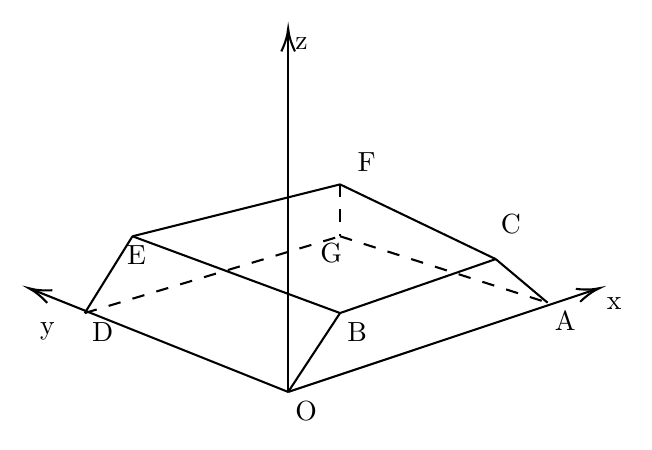
\begin{tikzpicture}[x=0.75pt,y=0.75pt,yscale=-1,xscale=1]
			\draw (250,250) -- (250,77) ;
			\draw [shift={(250,75)}, rotate = 90] [color={rgb, 255:red, 0; green, 0; blue, 0 }  ][line width=0.75]    (10.93,-3.29) .. controls (6.95,-1.4) and (3.31,-0.3) .. (0,0) .. controls (3.31,0.3) and (6.95,1.4) .. (10.93,3.29)   ;
			\draw    (250,250) -- (398.1,200.63) ;
			\draw [shift={(400,200)}, rotate = 161.57] [color={rgb, 255:red, 0; green, 0; blue, 0 }  ][line width=0.75]    (10.93,-3.29) .. controls (6.95,-1.4) and (3.31,-0.3) .. (0,0) .. controls (3.31,0.3) and (6.95,1.4) .. (10.93,3.29)   ;
			\draw    (250,250) -- (126.86,200.74) ;
			\draw [shift={(125,200)}, rotate = 21.8] [color={rgb, 255:red, 0; green, 0; blue, 0 }  ][line width=0.75]    (10.93,-3.29) .. controls (6.95,-1.4) and (3.31,-0.3) .. (0,0) .. controls (3.31,0.3) and (6.95,1.4) .. (10.93,3.29)   ;
			\draw  [dash pattern={on 4.5pt off 4.5pt}]  (152,212) -- (275,175) ;
			\draw  [dash pattern={on 4.5pt off 4.5pt}]  (275,175) -- (375,207) ;
			\draw    (175,175) -- (152,212) ;
			\draw    (175,175) -- (275,212) ;
			\draw    (250,250) -- (275,212) ;
			\draw    (275,212) -- (350,186) ;
			\draw    (350,186) -- (375,207) ;
			\draw    (175,175) -- (275,150) ;
			\draw    (275,150) -- (350,186) ;
			\draw  [dash pattern={on 4.5pt off 4.5pt}]  (275,150) -- (275,175) ;
			
			\draw (402,203) node [anchor=north west][inner sep=0.75pt]   [align=left] {x};
			
			\draw (129,215) node [anchor=north west][inner sep=0.75pt]   [align=left] {y};
			
			\draw (252,78) node [anchor=north west][inner sep=0.75pt]   [align=left] {z};
			
			\draw (252,253) node [anchor=north west][inner sep=0.75pt]   [align=left] {O};
			
			\draw (377,210) node [anchor=north west][inner sep=0.75pt]   [align=left] {A};
			
			\draw (154,215) node [anchor=north west][inner sep=0.75pt]   [align=left] {D};
			
			\draw (264,177) node [anchor=north west][inner sep=0.75pt]   [align=left] {G};
			
			\draw (177,178) node [anchor=north west][inner sep=0.75pt]   [ below] {E};
			
			\draw (277,215) node [anchor=north west][inner sep=0.75pt]   [align=left] {B};
			
			\draw (351,163) node [anchor=north west][inner sep=0.75pt]   [align=left] {C};
			
			\draw (282,133) node [anchor=north west][inner sep=0.75pt]   [align=left] {F};		
		\end{tikzpicture}
	\end{center}
	\shortans{$62{,}5$}
	\loigiai{Gắn hình chóp cụt $OAGD.BCFE$ vào hệ trục $Oxyz$, ta có: $O(0;0;0), A(100;0;0), G(100; 60;0), \\D(0;60;0), B(10;10;8)$, $\overrightarrow{OD}=(0 ; 60 ; 0), \overrightarrow{OB}=(10 ; 10 ; 8)$.\\
		Véc-tơ pháp tuyến của mặt phẳng $(OBED)$ là $\vec{n}=[\overrightarrow{OD}, \overrightarrow{OB}]=(480 ; 0 ;-600) = 120(4 ; 0 ;-5)$.\\
		Phương trình mặt phẳng $(OBED)$ đi qua điểm $O(0 ; 0 ; 0)$ và có véc-tơ pháp tuyến $\vec{n}=(4 ; 0 ;-5)$ là  $4x-5z=0$.\\
		Khoảng cách từ điểm $G$ đến mặt phẳng $(OBED)$ là $$\mathrm{d}(G,(O B E D))=\dfrac{|4\cdot 100-5\cdot 0|}{\sqrt{16+25}}=\dfrac{400 \sqrt{41}}{41} \approx 62{,}5.$$
	}
\end{ex}
\begin{ex}%[2H2V2-6]
	Một công trình đang xây dựng được gắn hệ trục $Oxyz$ như hình vẽ dưới (đơn vị trên mỗi trục tọa độ là mét). Mỗi cột bê tông có dạng hình lăng trụ tứ giác đều và có tâm của mặt đáy trên lần lợt là $A(3 ; 2 ; 3), B(6 ; 3 ; 3), C(9 ; 4 ; 2), D\left(6 ; 0 ; \dfrac{5}{2}\right)$. Tính khoảng cách từ điểm $D$ đến mặt phẳng $(ABC)$ (kết quả làm tròn tới hàng phần trăm).
	\begin{center}
		\includegraphics[width=0.5\linewidth]{image/h3.png}
	\end{center}
	\shortans{$2,85$}
	\loigiai{Ta có $\overrightarrow{AB}=(3;1;0); \overrightarrow{AC}=(6;2;-1)$. Phương trình mặt phẳng $(ABC)$ qua $A$ và có véc-tơ pháp tuyến $[\overrightarrow{AB},\overrightarrow{AC}]=(-1;3;0)$ là $-x + 3y - 3 = 0$. \\
		Khoảng cách từ $D$ tới mặt phẳng $(ABC)$ là $\mathrm{d}(D,(ABC))=\dfrac{\left|-6-3\right|}{\sqrt{1^2 + 3^2}}=\dfrac{9\sqrt{10}}{10} \approx 2{,}85$.
	}
\end{ex}

\begin{ex}%[2H2V2-6]
	Một công trình đang xây dựng được gắn hệ trục $Oxyz$ (đơn vị trên mỗi trục tọa độ là mét). Ba bức tường $(P),(Q),(R)$ (như hình vẽ) của tòa nhà lần lượt có phương trình $(P)\colon x+2y-2z+1=0$, $(Q)\colon 2x+y+2z-3=0,(R)\colon 2x+4y-4z-19=0$. Tính khoảng cách giữa hai bức tường $(P)$ và $(R)$ của tòa nhà.
	\begin{center}
		\includegraphics[width=0.5\linewidth]{image/h1.png}
	\end{center}
	\shortans{$3{,}5$}
	\loigiai{Tính khoảng cách giữa hai bức tường $(P)$ và $(R)$ của tòa nhà.\\
		Chọn điểm $M(-1 ; 0 ; 0) \in(P)$. Do hai bức tường $(P)$ và $(R)$ song song nhau nên \\
		$$\mathrm{d}((P),(R))=\mathrm{d}(M,(R))=\dfrac{|2\cdot (-1)+4\cdot 0-4\cdot 0-19|}{\sqrt{4+16+16}}=\dfrac{21}{6}=3{,}5 \text{m.}$$}
\end{ex}


\begin{ex}%[2H2V2-6]
	Một công trình đang xây dựng được gắn hệ trục $O x y z$ (đơn vị trên mỗi trục tọa độ là mét). Ba bức tường $(P),(Q),(R),(T)$ (như hình vẽ) của tòa nhà lần lượt có phương trình $(P)\colon 2x-y-z+1=0$, $(Q)\colon x+3y-z-2=0,(R)\colon 4x-2y-2 z+9=0,(T)\colon 2x+6y-2z+15=0$. Tính chiều rộng bức tường $(Q)$ của tòa nhà (kết quả làm tròn đến hàng phần chục).
	\begin{figure}[!ht]
		\centering
		\includegraphics[width=0.5\linewidth]{image/h2.png}
	\end{figure}
	\shortans{$2{,}9$}
	\loigiai{
		Do hai bức tường $(P)$ và $(R)$ song song nhau nên chiều rộng bức tường $(Q)$ là khoảng cách giữa hai bức tường $(P)$ và $(R)$. Chọn điểm $N(0 ; 0 ; 1) \in(P)$.\\
		Do hai bức tường $(P)$ và $(R)$ song song nhau nên $$\mathrm{d}((P),(R))=\mathrm{d}(N,(R))=\dfrac{|4\cdot 0-2\cdot 0-2\cdot 1+9|}{\sqrt{4+1+1}}=\dfrac{7}{\sqrt{6}} \approx 2{,}9.$$}
\end{ex}
\begin{ex}%[2H2V2-6]
	Cho hình lập phương $ABCD.A'B'C'D'$ có độ dài cạnh bằng 1. Gọi $M, N, P, Q$ lần lượt là trung điểm của $AB, BC, C'D',DD'$. Chọn hệ tọa độ $Oxyz$ như hình vẽ, xác định tọa độ các điểm $M, N, P, Q$. 
	Tính khoảng cách từ điểm $Q$ đến mặt phẳng $(MNP)$. Kết quả làm tròn đến hàng phần chục.
	\begin{center}
		\tikzset{every picture/.style={line width=0.75pt}} %set default line width to 0.75pt        
		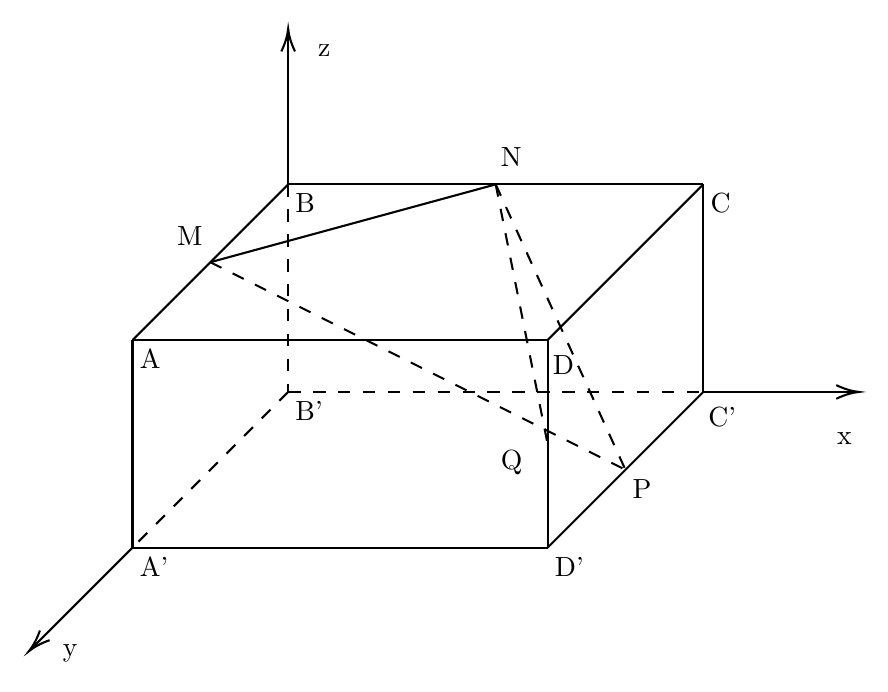
\begin{tikzpicture}[x=0.75pt,y=0.75pt,yscale=-1,xscale=1]
			%uncomment if require: \path (0,797); %set diagram left start at 0, and has height of 797
			%Straight Lines [id:da8382470567419189] 
			\draw    (250,400) -- (250,327) ;
			\draw [shift={(250,325)}, rotate = 90] [color={rgb, 255:red, 0; green, 0; blue, 0 }  ][line width=0.75]    (10.93,-3.29) .. controls (6.95,-1.4) and (3.31,-0.3) .. (0,0) .. controls (3.31,0.3) and (6.95,1.4) .. (10.93,3.29)   ;
			%Straight Lines [id:da22849660996364696] 
			\draw    (175,575) -- (375,575) ;
			%Straight Lines [id:da3429340193043935] 
			\draw    (375,575) -- (450,500) ;
			%Straight Lines [id:da6171158479105385] 
			\draw    (250,400) -- (175,475) ;
			%Straight Lines [id:da20159315767924957] 
			\draw    (175,475) -- (175,575) ;
			%Straight Lines [id:da09157475506424606] 
			\draw    (175,475) -- (375,475) ;
			%Straight Lines [id:da7794866428713987] 
			\draw    (375,475) -- (375,575) ;
			%Straight Lines [id:da5730802129402581] 
			\draw    (375,475) -- (450,400) ;
			%Straight Lines [id:da4069170044141508] 
			\draw    (250,400) -- (450,400) ;
			%Straight Lines [id:da7895384060713708] 
			\draw    (450,400) -- (450,500) ;
			%Straight Lines [id:da3822968918446086] 
			\draw    (212.5,437.5) -- (350,400) ;
			%Straight Lines [id:da5114427996681619] 
			\draw  [dash pattern={on 4.5pt off 4.5pt}]  (350,400) -- (412.5,537.5) ;
			%Straight Lines [id:da5639353335968631] 
			\draw  [dash pattern={on 4.5pt off 4.5pt}]  (212.5,437.5) -- (412.5,537.5) ;
			%Straight Lines [id:da7141193916967588] 
			\draw  [dash pattern={on 4.5pt off 4.5pt}]  (350,400) -- (375,525) ;
			%Straight Lines [id:da6592626042182406] 
			\draw  [dash pattern={on 4.5pt off 4.5pt}]  (250,500) -- (175,575) ;
			%Straight Lines [id:da4180570193860802] 
			\draw    (175,575) -- (126.41,623.59) ;
			\draw [shift={(125,625)}, rotate = 315] [color={rgb, 255:red, 0; green, 0; blue, 0 }  ][line width=0.75]    (10.93,-3.29) .. controls (6.95,-1.4) and (3.31,-0.3) .. (0,0) .. controls (3.31,0.3) and (6.95,1.4) .. (10.93,3.29)   ;
			%Straight Lines [id:da9167552187295651] 
			\draw  [dash pattern={on 4.5pt off 4.5pt}]  (250,500) -- (450,500) ;
			%Straight Lines [id:da8527980278686933] 
			\draw    (450,500) -- (523,500) ;
			\draw [shift={(525,500)}, rotate = 180] [color={rgb, 255:red, 0; green, 0; blue, 0 }  ][line width=0.75]    (10.93,-3.29) .. controls (6.95,-1.4) and (3.31,-0.3) .. (0,0) .. controls (3.31,0.3) and (6.95,1.4) .. (10.93,3.29)   ;
			%Straight Lines [id:da8000503760713495] 
			\draw  [dash pattern={on 4.5pt off 4.5pt}]  (250,400) -- (250,500) ;
			\draw (177,478) node [anchor=north west][inner sep=0.75pt]   [align=left] {A};
			
			\draw (252,403) node [anchor=north west][inner sep=0.75pt]   [align=left] {B};
			
			\draw (452,403) node [anchor=north west][inner sep=0.75pt]   [align=left] {C};
			
			\draw (376,481) node [anchor=north west][inner sep=0.75pt]   [align=left] {D};
			
			\draw (177,578) node [anchor=north west][inner sep=0.75pt]   [align=left] {A'};
			
			\draw (252,503) node [anchor=north west][inner sep=0.75pt]   [align=left] {B'};
			
			\draw (451,506) node [anchor=north west][inner sep=0.75pt]   [align=left] {C'};
			
			\draw (377,578) node [anchor=north west][inner sep=0.75pt]   [align=left] {D'};
			
			\draw (195,419) node [anchor=north west][inner sep=0.75pt]   [align=left] {M};
			
			\draw (351,381) node [anchor=north west][inner sep=0.75pt]   [align=left] {N};
			
			\draw (414.5,540.5) node [anchor=north west][inner sep=0.75pt]   [align=left] {P};
			
			\draw (351,527) node [anchor=north west][inner sep=0.75pt]   [align=left] {Q};
			
			\draw (513,518) node [anchor=north west][inner sep=0.75pt]   [align=left] {x};
			
			\draw (140,620) node [anchor=north west][inner sep=0.75pt]   [align=left] {y};
			
			\draw (263,331) node [anchor=north west][inner sep=0.75pt]   [align=left] {z};
		\end{tikzpicture}
	\end{center}
	\shortans{$1,4$}
	\loigiai{Thiết lập hệ tọa độ $O x y z$ như hình vẽ, gốc $O \equiv B'$. Khi đó $M\left(0 ; \dfrac{1}{2} ; 1\right), N\left(\dfrac{1}{2} ; 0 ; 1\right), P\left(1 ; \dfrac{1}{2} ; 0\right),\\
		Q\left(1 ; 1 ; \dfrac{1}{2}\right)$. Phương trình mặt phẳng $(MNP)$ đi qua $M\left(0;\dfrac{1}{2};1\right)$ và có véc-tơ pháp tuyến $[\overrightarrow {MN} ,\overrightarrow {MP}]=\left( \dfrac{1}{{2}};\dfrac{1}{{2}};\dfrac{1}{{2}}\right)$ là $2x + 2y + 2z - 3 = 0$.\\
		Khoảng cách từ điểm $Q$ đến mặt phẳng $(MNP)$ là $$\mathrm{d}(Q;(MNP)=\dfrac{\left|2\cdot 1+2\cdot 1+2\cdot \dfrac{1}{2}\right|}{\sqrt{2^2 +2^2 +2^2}}= \dfrac{5\sqrt{3}}{6}\approx 1{,}4.$$
	}
\end{ex}
\begin{ex}%[2H2V2-6]
	Cho hình chóp $S.ABCD$ có đáy $ABCD$ là hình vuông cạnh $a, SAD$ là tam giác đều và nằm trong mặt phẳng với đáy. Gọi $M$ và $N$ lần lượt là trung điểm của $BC$ và $CD$. Chọn hệ tọa độ $Oxyz$ như hình vẽ dưới. Gọi $Q$ là trung điểm $S D$. Tính khoảng cách giữa hai mặt phẳng $(SAC)$ và mặt phẳng $(ONQ)$ (kết quả làm tròn đến hàng phần chục).
	\begin{center}
		% Gradient Info
		\tikzset {_0pmvymc3o/.code = {\pgfsetadditionalshadetransform{ \pgftransformshift{\pgfpoint{-198 bp } { 158.4 bp }  }  \pgftransformscale{1.32 }  }}}
		\pgfdeclareradialshading{_ffechrcqo}{\pgfpoint{160bp}{-128bp}}{rgb(0bp)=(0,0,0);
			rgb(0bp)=(0,0,0);
			rgb(6.785714285714286bp)=(0,0,0);
			rgb(14.017857142857142bp)=(0,0,0);
			rgb(20bp)=(0,0,0);
			rgb(25bp)=(1,1,1);
			rgb(400bp)=(1,1,1)}
		\tikzset{every picture/.style={line width=0.75pt}} %set default line width to 0.75pt        
		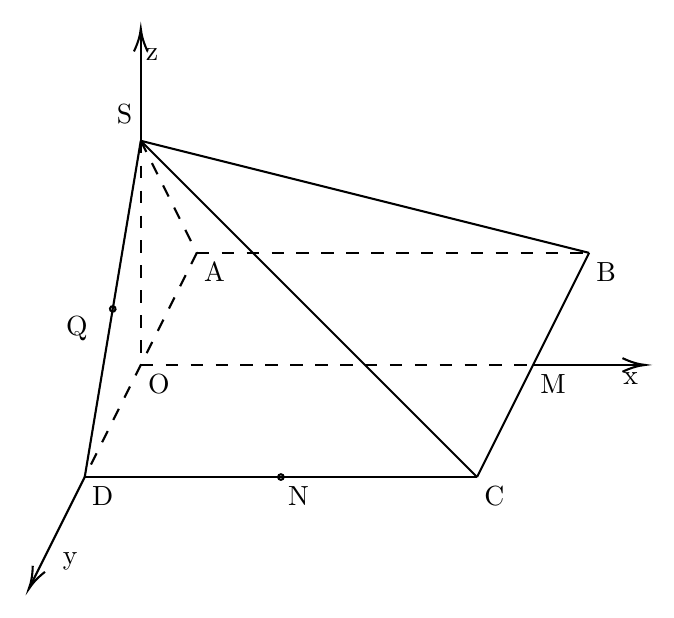
\begin{tikzpicture}[x=0.75pt,y=0.75pt,yscale=-1,xscale=1]
			%uncomment if require: \path (0,300); %set diagram left start at 0, and has height of 300
			%Straight Lines [id:da1986885226481041] 
			\draw    (108,216) -- (297,216) ;
			\draw [shift={(202.5,216)}, rotate = 0] [color={rgb, 255:red, 0; green, 0; blue, 0 }  ][line width=0.75]      (0, 0) circle [x radius= 1.34, y radius= 1.34]   ;
			%Straight Lines [id:da8495468285480916] 
			\draw [color={rgb, 255:red, 0; green, 0; blue, 0 }  ,draw opacity=1 ][shading=_ffechrcqo,_0pmvymc3o]   (135,54) -- (171,63) -- (207,72) -- (243,81) -- (279,90) -- (315,99) -- (351,108) ;
			%Straight Lines [id:da7064838767550801] 
			\draw  [dash pattern={on 4.5pt off 4.5pt}]  (135,162) -- (324,162) ;
			%Straight Lines [id:da7232875579325917] 
			\draw  [dash pattern={on 4.5pt off 4.5pt}]  (162,108) -- (108,216) ;
			%Straight Lines [id:da6308494004055998] 
			\draw  [dash pattern={on 4.5pt off 4.5pt}]  (162,108) -- (351,108) ;
			%Straight Lines [id:da6682204451648537] 
			\draw    (351,108) -- (297,216) ;
			%Straight Lines [id:da3749747303473572] 
			\draw  [dash pattern={on 4.5pt off 4.5pt}]  (135,54) -- (135,162) ;
			%Straight Lines [id:da8031053998975075] 
			\draw    (135,54) -- (108,216) ;
			\draw [shift={(121.5,135)}, rotate = 99.46] [color={rgb, 255:red, 0; green, 0; blue, 0 }  ][line width=0.75]      (0, 0) circle [x radius= 1.34, y radius= 1.34]   ;
			%Straight Lines [id:da6847944951979155] 
			\draw    (135,54) -- (297,216) ;
			%Straight Lines [id:da6134510126128467] 
			\draw  [dash pattern={on 4.5pt off 4.5pt}]  (135,54) -- (162,108) ;
			%Straight Lines [id:da8173261646582135] 
			\draw    (324,162) -- (376,162) ;
			\draw [shift={(378,162)}, rotate = 180] [color={rgb, 255:red, 0; green, 0; blue, 0 }  ][line width=0.75]    (10.93,-3.29) .. controls (6.95,-1.4) and (3.31,-0.3) .. (0,0) .. controls (3.31,0.3) and (6.95,1.4) .. (10.93,3.29)   ;
			%Straight Lines [id:da8552794618253725] 
			\draw    (108,216) -- (81.89,268.21) ;
			\draw [shift={(81,270)}, rotate = 296.57] [color={rgb, 255:red, 0; green, 0; blue, 0 }  ][line width=0.75]    (10.93,-3.29) .. controls (6.95,-1.4) and (3.31,-0.3) .. (0,0) .. controls (3.31,0.3) and (6.95,1.4) .. (10.93,3.29)   ;
			%Straight Lines [id:da44029097674743123] 
			\draw    (135,54) -- (135,2) ;
			\draw [shift={(135,0)}, rotate = 90] [color={rgb, 255:red, 0; green, 0; blue, 0 }  ][line width=0.75]    (10.93,-3.29) .. controls (6.95,-1.4) and (3.31,-0.3) .. (0,0) .. controls (3.31,0.3) and (6.95,1.4) .. (10.93,3.29)   ;
			\draw (164,111) node [anchor=north west][inner sep=0.75pt]   [align=left] {A};
			
			\draw (353,111) node [anchor=north west][inner sep=0.75pt]   [align=left] {B};
			
			\draw (299,219) node [anchor=north west][inner sep=0.75pt]   [align=left] {C};
			
			\draw (110,219) node [anchor=north west][inner sep=0.75pt]   [align=left] {D};
			
			\draw (326,165) node [anchor=north west][inner sep=0.75pt]   [align=left] {M};
			
			\draw (137,165) node [anchor=north west][inner sep=0.75pt]   [align=left] {O};
			
			\draw (204.5,219) node [anchor=north west][inner sep=0.75pt]   [align=left] {N};
			
			\draw (366,164) node [anchor=north west][inner sep=0.75pt]   [align=left] {x};
			
			\draw (96,251) node [anchor=north west][inner sep=0.75pt]   [align=left] {y};
			
			\draw (136,8) node [anchor=north west][inner sep=0.75pt]   [align=left] {z};
			
			\draw (122,35) node [anchor=north west][inner sep=0.75pt]   [align=left] {S};
			
			\draw (97.5,137) node [anchor=north west][inner sep=0.75pt]   [align=left] {Q};
		\end{tikzpicture}
	\end{center}
	\shortans{$0{,}3$}
	\loigiai{
		Với hệ trục toạ độ như hình vẽ ta có $S\left(0 ; 0 ; \dfrac{a \sqrt{3}}{2}\right) ; M(a ; 0 ; 0) ; N\left(\dfrac{a}{2} ; \dfrac{a}{2} ; 0\right); A(0;-\dfrac{a}{2};0);$\\
		$B\left(a;-\dfrac{-a}{2};0\right); C\left(a; \dfrac{a}{2};0\right); D\left(0;\dfrac{a}{2};0\right);Q\left(0;\dfrac{a}{4};\dfrac{a\sqrt{3}}{4}\right)$. \\
		Lấy $a=1.$ Mặt phẳng $(SAC)$ qua $A$ và có véc-tơ pháp tuyến $[\overrightarrow{SA},\overrightarrow{AC}]$ là
		$2\sqrt3 x - 2\sqrt3 y + 2z - \sqrt3 = 0.$\\
		Khoảng cách cần tìm 
		$$\mathrm{d}((SAC);(OQN))=\mathrm{d}(O;(SAC))= \dfrac{\sqrt{21}}{14}\approx 0{,}3.$$
	}
\end{ex}
\begin{ex}%[2H2V2-6]
	Cho tứ diện $OABC$, có $OA, OB, OC$ đôi một vuông góc và $OA=5, OB=2, OC=4$. Gọi $M, N$ lần lượt là trung điểm của $OB$ và $OC$. Chọn hệ tọa độ $Oxyz$ như hình vẽ dưới. Tính khoảng cách từ điểm $B$ đến mặt phẳng $(AMN)$. Kết quả làm tròn đến hàng phần chục.
	\begin{center}		
		
		\tikzset{every picture/.style={line width=0.75pt}} %set default line width to 0.75pt        
		
		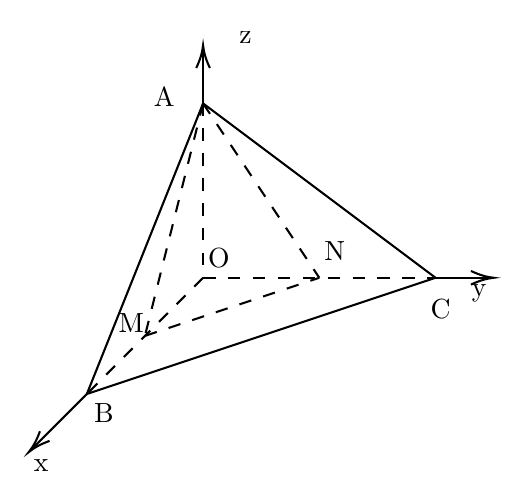
\begin{tikzpicture}[x=0.75pt,y=0.75pt,yscale=-1,xscale=1]
			%uncomment if require: \path (0,300); %set diagram left start at 0, and has height of 300
			
			%Straight Lines [id:da3679447504076472] 
			\draw  [dash pattern={on 4.5pt off 4.5pt}]  (252,140) -- (364,140) ;
			%Straight Lines [id:da13962597702284096] 
			\draw  [dash pattern={on 4.5pt off 4.5pt}]  (252,140) -- (196,196) ;
			%Straight Lines [id:da8580092790638094] 
			\draw  [dash pattern={on 4.5pt off 4.5pt}]  (252,56) -- (252,140) ;
			%Straight Lines [id:da7130062908773143] 
			\draw    (252,56) -- (196,196) ;
			%Straight Lines [id:da012778923343735649] 
			\draw    (252,56) -- (364,140) ;
			%Straight Lines [id:da3173437648870021] 
			\draw    (196,196) -- (364,140) ;
			%Straight Lines [id:da528126976168177] 
			\draw  [dash pattern={on 4.5pt off 4.5pt}]  (224,168) -- (308,140) ;
			%Straight Lines [id:da44405621585220234] 
			\draw  [dash pattern={on 4.5pt off 4.5pt}]  (252,56) -- (308,140) ;
			%Straight Lines [id:da4474952587057264] 
			\draw  [dash pattern={on 4.5pt off 4.5pt}]  (252,56) -- (224,168) ;
			%Straight Lines [id:da6666103459826491] 
			\draw    (252,56) -- (252,30) ;
			\draw [shift={(252,28)}, rotate = 90] [color={rgb, 255:red, 0; green, 0; blue, 0 }  ][line width=0.75]    (10.93,-3.29) .. controls (6.95,-1.4) and (3.31,-0.3) .. (0,0) .. controls (3.31,0.3) and (6.95,1.4) .. (10.93,3.29)   ;
			%Straight Lines [id:da6450164393512425] 
			\draw    (364,140) -- (390,140) ;
			\draw [shift={(392,140)}, rotate = 180] [color={rgb, 255:red, 0; green, 0; blue, 0 }  ][line width=0.75]    (10.93,-3.29) .. controls (6.95,-1.4) and (3.31,-0.3) .. (0,0) .. controls (3.31,0.3) and (6.95,1.4) .. (10.93,3.29)   ;
			%Straight Lines [id:da9897161761780247] 
			\draw    (196,196) -- (169.41,222.59) ;
			\draw [shift={(168,224)}, rotate = 315] [color={rgb, 255:red, 0; green, 0; blue, 0 }  ][line width=0.75]    (10.93,-3.29) .. controls (6.95,-1.4) and (3.31,-0.3) .. (0,0) .. controls (3.31,0.3) and (6.95,1.4) .. (10.93,3.29)   ;
			
			
			\draw (169,226) node [anchor=north west][inner sep=0.75pt]   [align=left] {x};
			
			\draw (380,142) node [anchor=north west][inner sep=0.75pt]   [align=left] {y};
			
			\draw (268,20) node [anchor=north west][inner sep=0.75pt]   [align=left] {z};
			
			\draw (226.8,46.8) node [anchor=north west][inner sep=0.75pt]   [align=left] {A};
			
			\draw (198,199) node [anchor=north west][inner sep=0.75pt]   [align=left] {B};
			
			\draw (360.2,149) node [anchor=north west][inner sep=0.75pt]   [align=left] {C};
			
			\draw (253,124.6) node [anchor=north west][inner sep=0.75pt]   [align=left] {O};
			
			\draw (209.8,155.6) node [anchor=north west][inner sep=0.75pt]   [align=left] {M};
			
			\draw (309,121) node [anchor=north west][inner sep=0.75pt]   [align=left] {N};
			
			
		\end{tikzpicture}
	\end{center}	
	\shortans{$0{,}9$}
	\loigiai{Chọn hệ trục tọa độ Oxyz như hình vẽ.
		
		\begin{center}
			
			\tikzset{every picture/.style={line width=0.75pt}} %set default line width to 0.75pt        
			
			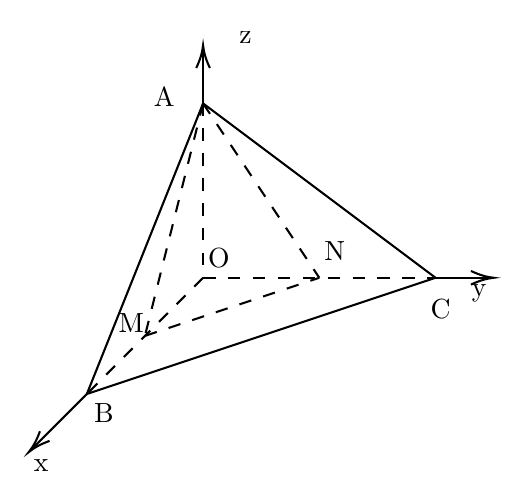
\begin{tikzpicture}[x=0.75pt,y=0.75pt,yscale=-1,xscale=1]
				
				
				%Straight Lines [id:da3679447504076472] 
				\draw  [dash pattern={on 4.5pt off 4.5pt}]  (252,140) -- (364,140) ;
				%Straight Lines [id:da13962597702284096] 
				\draw  [dash pattern={on 4.5pt off 4.5pt}]  (252,140) -- (196,196) ;
				%Straight Lines [id:da8580092790638094] 
				\draw  [dash pattern={on 4.5pt off 4.5pt}]  (252,56) -- (252,140) ;
				%Straight Lines [id:da7130062908773143] 
				\draw    (252,56) -- (196,196) ;
				%Straight Lines [id:da012778923343735649] 
				\draw    (252,56) -- (364,140) ;
				%Straight Lines [id:da3173437648870021] 
				\draw    (196,196) -- (364,140) ;
				%Straight Lines [id:da528126976168177] 
				\draw  [dash pattern={on 4.5pt off 4.5pt}]  (224,168) -- (308,140) ;
				%Straight Lines [id:da44405621585220234] 
				\draw  [dash pattern={on 4.5pt off 4.5pt}]  (252,56) -- (308,140) ;
				%Straight Lines [id:da4474952587057264] 
				\draw  [dash pattern={on 4.5pt off 4.5pt}]  (252,56) -- (224,168) ;
				%Straight Lines [id:da6666103459826491] 
				\draw    (252,56) -- (252,30) ;
				\draw [shift={(252,28)}, rotate = 90] [color={rgb, 255:red, 0; green, 0; blue, 0 }  ][line width=0.75]    (10.93,-3.29) .. controls (6.95,-1.4) and (3.31,-0.3) .. (0,0) .. controls (3.31,0.3) and (6.95,1.4) .. (10.93,3.29)   ;
				%Straight Lines [id:da6450164393512425] 
				\draw    (364,140) -- (390,140) ;
				\draw [shift={(392,140)}, rotate = 180] [color={rgb, 255:red, 0; green, 0; blue, 0 }  ][line width=0.75]    (10.93,-3.29) .. controls (6.95,-1.4) and (3.31,-0.3) .. (0,0) .. controls (3.31,0.3) and (6.95,1.4) .. (10.93,3.29)   ;
				%Straight Lines [id:da9897161761780247] 
				\draw    (196,196) -- (169.41,222.59) ;
				\draw [shift={(168,224)}, rotate = 315] [color={rgb, 255:red, 0; green, 0; blue, 0 }  ][line width=0.75]    (10.93,-3.29) .. controls (6.95,-1.4) and (3.31,-0.3) .. (0,0) .. controls (3.31,0.3) and (6.95,1.4) .. (10.93,3.29)   ;
				
				
				\draw (169,226) node [anchor=north west][inner sep=0.75pt]   [align=left] {x};
				
				\draw (380,142) node [anchor=north west][inner sep=0.75pt]   [align=left] {y};
				
				\draw (268,20) node [anchor=north west][inner sep=0.75pt]   [align=left] {z};
				
				\draw (226.8,46.8) node [anchor=north west][inner sep=0.75pt]   [align=left] {A};
				
				\draw (198,199) node [anchor=north west][inner sep=0.75pt]   [align=left] {B};
				
				\draw (360.2,149) node [anchor=north west][inner sep=0.75pt]   [align=left] {C};
				
				\draw (253,124.6) node [anchor=north west][inner sep=0.75pt]   [align=left] {O};
				
				\draw (209.8,155.6) node [anchor=north west][inner sep=0.75pt]   [align=left] {M};
				
				\draw (309,121) node [anchor=north west][inner sep=0.75pt]   [align=left] {N};
				
				
			\end{tikzpicture}
		\end{center}
		Ta có $O(0 ; 0 ; 0), A \in {Oz}, B \in O x, C \in O y$ sao cho $A O=5, OB=2, OC=4\Rightarrow A(0 ; 0 ; 5), B(2 ; 0 ; 0), C(0 ; 4 ; 0)$. $M$ là trung điểm $OB$ nên $M(1 ; 0 ; 0)$. $N$ là trung điểm $OC$ nên $N(0 ; 2 ; 0)$.\\
		Phương trình mặt phẳng $(AMN)$ qua $A$ và có véc-tơ pháp tuyến $[\overrightarrow{AM},\overrightarrow{AN}]=(10;5;2)$ là $10x + 5y + 2z - 10 = 0$.\\
		Ta có $\mathrm{d}(B;(AMN))=\mathrm{d}(O;(AMN))=\dfrac{10}{\sqrt{129}}\approx 0{,}9$.
		
	}
\end{ex}

\begin{ex}%[2H2V2-6]
	Cho hình chóp $S.ABCD$ đáy là hình thang vuông tại $A$ và $D, SA \perp(ABCD)$. Góc giữa $SB$ và mặt phẳng đáy bằng $45^{\circ}, E$ là trung điểm của $SD, AB=2a, AD = DC = a$. Chọn hệ tọa độ $Oxyz$ như hình vẽ dưới. Tính khoảng cách từ điểm $B$ đến mặt phẳng $(AEC)$ (kết quả làm tròn đến hàng phần chục).
	\begin{center}	
		
		\tikzset{every picture/.style={line width=0.75pt}} %set default line width to 0.75pt        
		
		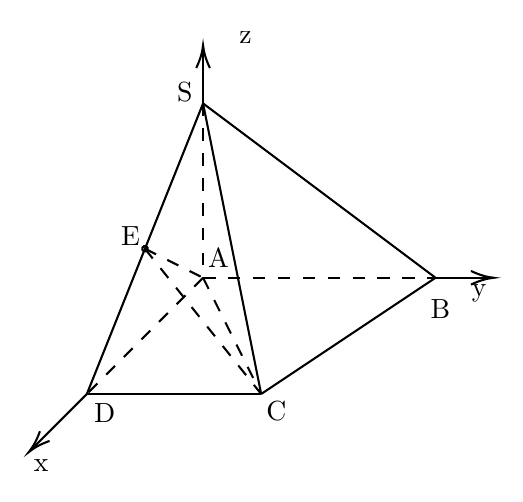
\begin{tikzpicture}[x=0.75pt,y=0.75pt,yscale=-1,xscale=1]
			%uncomment if require: \path (0,300); %set diagram left start at 0, and has height of 300
			
			%Straight Lines [id:da8913682824234928] 
			\draw  [dash pattern={on 4.5pt off 4.5pt}]  (252,140) -- (364,140) ;
			%Straight Lines [id:da039948733048584595] 
			\draw  [dash pattern={on 4.5pt off 4.5pt}]  (252,140) -- (196,196) ;
			%Straight Lines [id:da6718633500675624] 
			\draw  [dash pattern={on 4.5pt off 4.5pt}]  (252,56) -- (252,140) ;
			%Straight Lines [id:da9759242944770992] 
			\draw    (252,56) -- (196,196) ;
			\draw [shift={(224,126)}, rotate = 111.8] [color={rgb, 255:red, 0; green, 0; blue, 0 }  ][line width=0.75]      (0, 0) circle [x radius= 1.34, y radius= 1.34]   ;
			%Straight Lines [id:da563221306551871] 
			\draw    (252,56) -- (364,140) ;
			%Straight Lines [id:da15516892739193677] 
			\draw    (280,196) -- (364,140) ;
			%Straight Lines [id:da7881469638756575] 
			\draw    (252,56) -- (252,30) ;
			\draw [shift={(252,28)}, rotate = 90] [color={rgb, 255:red, 0; green, 0; blue, 0 }  ][line width=0.75]    (10.93,-3.29) .. controls (6.95,-1.4) and (3.31,-0.3) .. (0,0) .. controls (3.31,0.3) and (6.95,1.4) .. (10.93,3.29)   ;
			%Straight Lines [id:da6714011604516419] 
			\draw    (364,140) -- (390,140) ;
			\draw [shift={(392,140)}, rotate = 180] [color={rgb, 255:red, 0; green, 0; blue, 0 }  ][line width=0.75]    (10.93,-3.29) .. controls (6.95,-1.4) and (3.31,-0.3) .. (0,0) .. controls (3.31,0.3) and (6.95,1.4) .. (10.93,3.29)   ;
			%Straight Lines [id:da5385347511589023] 
			\draw    (196,196) -- (169.41,222.59) ;
			\draw [shift={(168,224)}, rotate = 315] [color={rgb, 255:red, 0; green, 0; blue, 0 }  ][line width=0.75]    (10.93,-3.29) .. controls (6.95,-1.4) and (3.31,-0.3) .. (0,0) .. controls (3.31,0.3) and (6.95,1.4) .. (10.93,3.29)   ;
			%Straight Lines [id:da05923631932446871] 
			\draw    (196,196) -- (280,196) ;
			%Straight Lines [id:da8592722804571848] 
			\draw    (252,56) -- (280,196) ;
			%Straight Lines [id:da802931795948812] 
			\draw  [dash pattern={on 4.5pt off 4.5pt}]  (252,140) -- (280,196) ;
			%Straight Lines [id:da4994838123991385] 
			\draw  [dash pattern={on 4.5pt off 4.5pt}]  (224,126) -- (252,140) ;
			%Straight Lines [id:da23640159060964017] 
			\draw  [dash pattern={on 4.5pt off 4.5pt}]  (224,126) -- (280,196) ;
			
			
			\draw (169,226) node [anchor=north west][inner sep=0.75pt]   [align=left] {x};
			
			\draw (380,142) node [anchor=north west][inner sep=0.75pt]   [align=left] {y};
			
			\draw (268,20) node [anchor=north west][inner sep=0.75pt]   [align=left] {z};
			
			\draw (238,44.4) node [anchor=north west][inner sep=0.75pt]   [align=left] {S};
			
			\draw (198,199) node [anchor=north west][inner sep=0.75pt]   [align=left] {D};
			
			\draw (360.2,149) node [anchor=north west][inner sep=0.75pt]   [align=left] {B};
			
			\draw (253,124.6) node [anchor=north west][inner sep=0.75pt]   [align=left] {A};
			
			\draw (281,198) node [anchor=north west][inner sep=0.75pt]   [align=left] {C};
			
			\draw (211,114) node [anchor=north west][inner sep=0.75pt]   [align=left] {E};
			
			
		\end{tikzpicture}
	\end{center}
	\shortans{$1{,}3$}
	\loigiai{Lấy $a=1$. Ta có $(SB,(ABCD))=\widehat{SBA}=45^0 \Rightarrow \triangle ASB$ vuông cân tại $A.$ Suy ra $SA=AB=2$.\\
		Ta có $A(0;0;0); S(0;0;2); C(1;1;0); B(0;2;0); D(1;0;0); E\left(\dfrac{1}{2};0;1\right)$.\\
		Phương trình mặt phẳng $(AEC)$ qua $A$ và có véc-tơ pháp tuyến $[\overrightarrow{AE}, \overrightarrow{AC}]=\left(-1;1;\dfrac{1}{2}\right)$ là $-2x + 2y + z = 0$.\\
		Khoảng cách từ điểm $B$ đến mặt phẳng $(AEC)$ là 
		$$\mathrm{d}(B,(AEC))=\dfrac{|2\cdot 2|}{\sqrt{2^2 +2^2 +1^2}}=\dfrac{4}{3}\approx 1{,}3.$$}
\end{ex}

\begin{ex}%[2H2V2-6]
	Trong không gian với hệ trục tọa độ $Oxyz$, cho bốn điểm $S(-1 ; 6 ; 2), A(0 ; 0 ; 6),\\ B(0 ; 3 ; 0)$, $C(-2 ; 0 ; 0)$. Gọi $H$ là chân đường cao vẽ từ $S$ của tứ diện $S.ABC$. Giả sử phương trình mặt phẳng đi qua ba điểm $S,B,H$ có dạng $x+by+cz+d=0$ với $b,c,d \in \mathbb{Z}$. Tính $b+c+d.$
	\shortans{$-17$}
	\loigiai{Phương trình mặt phẳng $(ABC): \dfrac{x}{-2}+\dfrac{y}{3}+\dfrac{z}{6}=1 \Leftrightarrow-3 x+2 y+z-6=0$. \\
		$H$ là chân đường cao vẽ từ $S$ của tứ diện $S.ABC$ nên $H$ là hình chiếu vuông góc của $S$ lên mặt phẳng $(A B C) \Rightarrow H\left(\dfrac{19}{14} ; \dfrac{31}{7} ; \dfrac{17}{14}\right)$.\\
		Mặt phẳng $(SBH)$ qua $B(0;3;0)$ và có véc-tơ pháp tuyến $$[\overrightarrow{BH}, \overrightarrow{SB}]=\left(\dfrac{11}{14} ; \dfrac{55}{14} ;-\dfrac{11}{2}\right)=\dfrac{11}{14}(1 ; 5 ;-7).$$
		Phương trình mặt phẳng $(SBH)$ là $ x+5(y-3)-7 z=0\\ \Leftrightarrow x+5 y-7 z-15=0$. Ta có $b+c+d =-17.$
	}
\end{ex}
\begin{ex}%[2H2V2-6]
	Trong KG $Oxyz$, cho hình chóp $S.ABCD$, đáy $ABCD$ là hình chữ nhật. Biết $A(0 ; 0 ; 0), D(2 ; 0 ; 0), B(0 ; 4 ; 0), S(0 ; 0 ; 4)$. Gọi $M$ là trung điểm của $SB$ và $G$ là trọng tâm của tam giác $SCD$. Tính khoảng cách từ điểm $B$ đến mặt phẳng $(AMG)$. Kết quả làm tròn đến hàng phần chục.
	\shortans{$2{,}8$}
	\loigiai{
		\begin{center}
			\tikzset{every picture/.style={line width=0.75pt}} %set default line width to 0.75pt        
			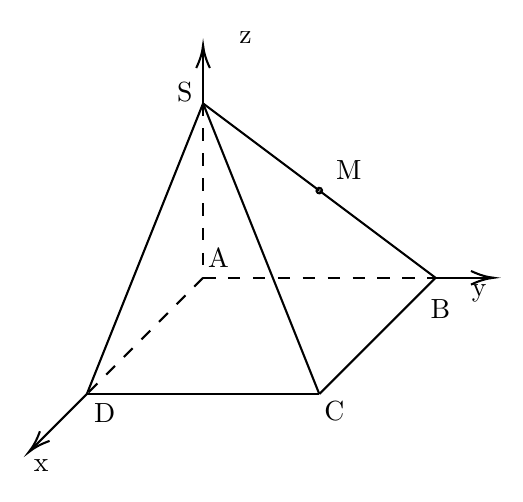
\begin{tikzpicture}[x=0.75pt,y=0.75pt,yscale=-1,xscale=1]
				%uncomment if require: \path (0,300); %set diagram left start at 0, and has height of 300
				
				%Straight Lines [id:da8697087570722153] 
				\draw  [dash pattern={on 4.5pt off 4.5pt}]  (252,140) -- (364,140) ;
				%Straight Lines [id:da4072889759548881] 
				\draw  [dash pattern={on 4.5pt off 4.5pt}]  (252,140) -- (196,196) ;
				%Straight Lines [id:da5044623873055065] 
				\draw  [dash pattern={on 4.5pt off 4.5pt}]  (252,56) -- (252,140) ;
				%Straight Lines [id:da6764918883827946] 
				\draw    (252,56) -- (196,196) ;
				%Straight Lines [id:da4329647923634008] 
				\draw    (252,56) -- (308,98) ;
				%Straight Lines [id:da011038461362765872] 
				\draw    (308.27,98.2) -- (364,140) ;
				\draw [shift={(308,98)}, rotate = 36.87] [color={rgb, 255:red, 0; green, 0; blue, 0 }  ][line width=0.75]      (0, 0) circle [x radius= 1.34, y radius= 1.34]   ;
				%Straight Lines [id:da5196781175343534] 
				\draw    (308,196) -- (364,140) ;
				%Straight Lines [id:da3160409919917737] 
				\draw    (252,56) -- (252,30) ;
				\draw [shift={(252,28)}, rotate = 90] [color={rgb, 255:red, 0; green, 0; blue, 0 }  ][line width=0.75]    (10.93,-3.29) .. controls (6.95,-1.4) and (3.31,-0.3) .. (0,0) .. controls (3.31,0.3) and (6.95,1.4) .. (10.93,3.29)   ;
				%Straight Lines [id:da9102255389540188] 
				\draw    (364,140) -- (390,140) ;
				\draw [shift={(392,140)}, rotate = 180] [color={rgb, 255:red, 0; green, 0; blue, 0 }  ][line width=0.75]    (10.93,-3.29) .. controls (6.95,-1.4) and (3.31,-0.3) .. (0,0) .. controls (3.31,0.3) and (6.95,1.4) .. (10.93,3.29)   ;
				%Straight Lines [id:da3969763351140396] 
				\draw    (196,196) -- (169.41,222.59) ;
				\draw [shift={(168,224)}, rotate = 315] [color={rgb, 255:red, 0; green, 0; blue, 0 }  ][line width=0.75]    (10.93,-3.29) .. controls (6.95,-1.4) and (3.31,-0.3) .. (0,0) .. controls (3.31,0.3) and (6.95,1.4) .. (10.93,3.29)   ;
				%Straight Lines [id:da06997294598351322] 
				\draw    (196,196) -- (308,196) ;
				%Straight Lines [id:da06948427828035464] 
				\draw    (252,56) -- (308,196) ;
				
				
				\draw (169,226) node [anchor=north west][inner sep=0.75pt]   [align=left] {x};
				
				\draw (380,142) node [anchor=north west][inner sep=0.75pt]   [align=left] {y};
				
				\draw (268,20) node [anchor=north west][inner sep=0.75pt]   [align=left] {z};
				
				\draw (238,44.4) node [anchor=north west][inner sep=0.75pt]   [align=left] {S};
				
				\draw (198,199) node [anchor=north west][inner sep=0.75pt]   [align=left] {D};
				
				\draw (360.2,149) node [anchor=north west][inner sep=0.75pt]   [align=left] {B};
				
				\draw (253,124.6) node [anchor=north west][inner sep=0.75pt]   [align=left] {A};
				
				\draw (309,198) node [anchor=north west][inner sep=0.75pt]   [align=left] {C};
				
				\draw (314.6,82) node [anchor=north west][inner sep=0.75pt]   [align=left] {M};
			\end{tikzpicture}
		\end{center}
		Chọn hệ trục tọa độ như hình vẽ. Ta có $A(0 ; 0 ; 0), D(2 ; 0 ; 0), B(0 ; 4 ; 0), S(0 ; 0 ; 4)$.\\
		$M$ là trung điểm của $S B \Rightarrow M(0 ; 2 ; 2)$.\\
		Tứ giác $A B C D$ là hình chữ nhật nên $\left\{\begin{array}{l}x_{A}+x_{C}=x_{B}+x_{D} \\ y_{A}+y_{C}=y_{B}+y_{D} \\ z_{A}+z_{C}=z_{B}+z_{D}\end{array} \Rightarrow\left\{\begin{array}{l}x_{C}=2 \\ y_{C}=4 \\ z_{C}=0\end{array} \Rightarrow C(2 ; 4 ; 0)\right.\right.$.\\
		$G$ là trọng tâm của tam giác $S C D \Rightarrow G\left(\dfrac{4}{3}; \dfrac{4}{3} ; \dfrac{4}{3}\right)$.\\
		Phương trình mặt phẳng $(AMG)$ qua $A$ và có véc-tơ pháp tuyến $[\overrightarrow{AM},\overrightarrow{AG}]=\left(0;\dfrac{-8}{3};\dfrac{8}{3} \right)$ là $y-z=0.$\\
		Khoảng cách từ điểm B đến mặt phẳng $(AMG)$ là $\mathrm{d}(B,(AMG))= \dfrac{|4|}{\sqrt{1^2+1^2}}=\dfrac{4}{\sqrt{2}}\approx 2{,}8$.
	}
\end{ex}

\begin{ex}%[2H2V2-6]
	Cho hình hộp chữ nhật $ABCD \cdot A'B'C'D'$ có các kích thước $AB=4, AD=3, AA'=5$. Gọi $G$ là trọng tâm của tam giác $ACB'$. Gọi $m$ là khoảng cách từ điểm $G$ đến mặt phẳng $\left(AB'C\right)$ và $n$ là khoảng cách giữa hai mặt phẳng $(AB'D')$ và $(CB'D')$. Tính $m+n$.
	\shortans{$0$}
	\loigiai{
		\begin{center}
			\tikzset{every picture/.style={line width=0.75pt}} %set default line width to 0.75pt        
			\begin{tikzpicture}[x=0.75pt,y=0.75pt,yscale=-1,xscale=1]
				%Straight Lines [id:da09989011048457908] 
				\draw    (250,400) -- (250,327) ;
				\draw [shift={(250,325)}, rotate = 90] [color={rgb, 255:red, 0; green, 0; blue, 0 }  ][line width=0.75]    (10.93,-3.29) .. controls (6.95,-1.4) and (3.31,-0.3) .. (0,0) .. controls (3.31,0.3) and (6.95,1.4) .. (10.93,3.29)   ;
				%Straight Lines [id:da5887885003342179] 
				\draw    (175,575) -- (375,575) ;
				%Straight Lines [id:da38181530618442316] 
				\draw    (375,575) -- (450,500) ;
				%Straight Lines [id:da5520368192051237] 
				\draw    (250,400) -- (175,475) ;
				%Straight Lines [id:da857881333421624] 
				\draw    (175,475) -- (175,575) ;
				%Straight Lines [id:da1055531864002952] 
				\draw    (175,475) -- (375,475) ;
				%Straight Lines [id:da9921967082690255] 
				\draw    (375,475) -- (375,575) ;
				%Straight Lines [id:da830188535856651] 
				\draw    (375,475) -- (450,400) ;
				%Straight Lines [id:da8543854930333936] 
				\draw    (250,400) -- (450,400) ;
				%Straight Lines [id:da010540648916782303] 
				\draw    (450,400) -- (450,500) ;
				%Straight Lines [id:da5916479203423954] 
				\draw  [dash pattern={on 4.5pt off 4.5pt}]  (250,500) -- (175,575) ;
				%Straight Lines [id:da3953089475850997] 
				\draw    (175,575) -- (126.41,623.59) ;
				\draw [shift={(125,625)}, rotate = 315] [color={rgb, 255:red, 0; green, 0; blue, 0 }  ][line width=0.75]    (10.93,-3.29) .. controls (6.95,-1.4) and (3.31,-0.3) .. (0,0) .. controls (3.31,0.3) and (6.95,1.4) .. (10.93,3.29)   ;
				%Straight Lines [id:da9157272689802225] 
				\draw  [dash pattern={on 4.5pt off 4.5pt}]  (250,500) -- (450,500) ;
				%Straight Lines [id:da9303391433588712] 
				\draw    (450,500) -- (523,500) ;
				\draw [shift={(525,500)}, rotate = 180] [color={rgb, 255:red, 0; green, 0; blue, 0 }  ][line width=0.75]    (10.93,-3.29) .. controls (6.95,-1.4) and (3.31,-0.3) .. (0,0) .. controls (3.31,0.3) and (6.95,1.4) .. (10.93,3.29)   ;
				%Straight Lines [id:da1786416964548232] 
				\draw  [dash pattern={on 4.5pt off 4.5pt}]  (250,400) -- (250,500) ;
				\draw (177,478) node [anchor=north west][inner sep=0.75pt]   [align=left] {D'};
				
				\draw (252,403) node [anchor=north west][inner sep=0.75pt]   [align=left] {A'};
				
				\draw (452,403) node [anchor=north west][inner sep=0.75pt]   [align=left] {B'};
				
				\draw (376,481) node [anchor=north west][inner sep=0.75pt]   [align=left] {C'};
				
				\draw (177,578) node [anchor=north west][inner sep=0.75pt]   [align=left] {D};
				
				\draw (252,503) node [anchor=north west][inner sep=0.75pt]   [align=left] {A};
				
				\draw (452,503) node [anchor=north west][inner sep=0.75pt]   [align=left] {B};
				
				\draw (377,578) node [anchor=north west][inner sep=0.75pt]   [align=left] {C};
				
				\draw (513,518) node [anchor=north west][inner sep=0.75pt]   [align=left] {x};
				
				\draw (140,620) node [anchor=north west][inner sep=0.75pt]   [align=left] {y};
				
				\draw (263,331) node [anchor=north west][inner sep=0.75pt]   [align=left] {z};
			\end{tikzpicture}
		\end{center}			
		Chọn hệ trục tọa độ như hình vẽ. Ta có $A(0;0 ; 0), C(4 ; 3 ; 0), B^{\prime}(4 ; 0 ; 5), B(4 ; 0 ; 0); D'(0;3;5).$ $G$ là trọng tâm của tam giác $ACB' \Rightarrow G\left(\dfrac{8}{3} ; 1 ; \dfrac{5}{3}\right).$\\
		Vì $G \in (ACB')$ nên $\mathrm{d}(G, (ACB'))=0.$\\
		Vì hai mặt phẳng $(AB'D')$ và $(CB'D')$ cắt nhau nên khoảng cách của chúng  bằng $0.$ \\
		Vậy $m+n=0$.}
\end{ex}
\Closesolutionfile{ans}
\indapan{6}{ans/ans-0-B15-KQ}

%%%==============Bai_BT1==============%%%
\begin{ex}%[2H5C1-5]
	Cho hình chóp $S.ABCD$ có đáy $ABCD$ là hình vuông cạnh $a$, cạnh bên $SA=a$ và vuông góc với mặt phẳng đáy. Gọi $M$, $N$ lần lượt là trung điểm của $SB$ và $SD$ và $G$ là trọng tâm của tam giác $AMN$.  Biết độ dài đoạn $BG$ có dạng $x\cdot a$. Hỏi giá trị $x$ bằng bao nhiêu? (Kết quả được làm tròn đến hàng phần trăm).
	
	\shortans{$0{,}87$}
	\loigiai{
		\immini{Đặt hệ trục tọa độ $Oxyz$ như hình vẽ. Khi đó\\ 
			$A\equiv O (0;0;0)$, $B\left(a;0;0\right)$, $D\left(0;a;0\right)$, $S\left(0;0;a\right)$.\\ 
			Suy ra $M\left(\dfrac{a}{2};0;\dfrac{a}{2} \right)$ và $N\left(0;\dfrac{a}{2};\dfrac{a}{2} \right)$.\\
			Vì $G$ là trọng tâm của tam giác $AMN$ nên $G\left(\dfrac{a}{6};\dfrac{a}{6};\dfrac{a}{3} \right)$.\\
			Khi đó độ dài đoạn $BG$ là
			$$BG=\sqrt{\left(\dfrac{5a}{6}\right)^2+\left(\dfrac{a}{6}\right)^2+\left(\dfrac{a}{6}\right)^2}=\dfrac{\sqrt{3}}{2}a\approx 0{,}87 a.$$}{\begin{tikzpicture}[scale=0.9]
				\def\a{3.5}
				\def\h{3.5}
				\path 	(0:0) coordinate (A)
				++(0:\a) coordinate (D)
				++(-130:\a/2) coordinate (C)
				($(A)+(C)-(D)$) coordinate (B)
				($(A)+(90:\h)$) coordinate (S)
				(intersection of A--C and B--D) coordinate (O)
				($(S)!0.5!(B)$) coordinate (M)
				($(S)!0.5!(D)$) coordinate (N)
				($(M)!0.5!(N)$) coordinate (I)
				($(A)!2/3!(I)$) coordinate (G);
				\draw[dashed,thick] 	(B)--(A)--(D)	(A)--(S) (A)--(M)--(N)--(A) (B)--(D);
				\draw [-stealth,thick]  (B) -- ($(B)!-1/2!(A)$)node[left, below]{$x$};	
				\draw [-stealth,thick]  (S) -- ($(S)!-1/3!(A)$)node[above]{$z$};
				\draw [-stealth,thick]  (D) -- ($(D)!-1/4!(A)$)node[right]{$y$};
				\draw[thick] 			(B)--(C)--(D)
				(B)--(S)	(C)--(S)	(D)--(S);
				\foreach \x/\g in {A/-65,B/150,C/-45,D/45,S/180,M/150,N/20,G/0}
				\fill[black] 	(\x) circle (1.5pt)
				($(\g:3mm)+(\x)$) node {$\x$};
		\end{tikzpicture}}
	}
\end{ex}
%%%==============HetBai_BT1==============%%%

%%%==============Bai_BT2==============%%%
\begin{ex}%[2H5C1-5]
	Cho hình chóp $S.ABCD$ có đáy $ABCD$ là hình vuông cạnh $a$, cạnh bên $SA=a$ và vuông góc với mặt phẳng đáy. Gọi $M$, $N$ lần lượt là trung điểm của $SB$ và $SD$ và $G$ là trọng tâm của tam giác $AMN$. Khoảng cách từ điểm $G$ đến mặt phẳng $\left(SBC\right)$ là bao nhiêu nếu $a=6\sqrt{3}$?
	
	\shortans{$2$}
	\loigiai{
		\immini{Chọn hệ trục tọa độ $Oxyz$ thỏa mãn:\\ 
			$A\equiv O(0;0;0)$, $B\left(a;0;0\right)$, $D\left(0;a;0\right)$, $S\left(0;0;a\right)$.\\ 
			Do đó $C(a;a;0)$.\\ 
			Suy ra $M\left(\dfrac{a}{2};0;\dfrac{a}{2} \right)$ và $N\left(0;\dfrac{a}{2};\dfrac{a}{2} \right)$.\\
			Vì $G$ là trọng tâm của tam giác $AMN$ nên $G\left(\dfrac{a}{6};\dfrac{a}{6};\dfrac{a}{3} \right)$.\\
			Phương trình mặt phẳng $(SBD)$ là 
			$$\dfrac{x}{a}+\dfrac{y}{a}+\dfrac{z}{a}=1.$$
			Do đó khoảng cách từ $G$ đến mặt phẳng $\left(SBC\right)$ là
			$$\mathrm{d}\left(G,(SBD)\right)=\dfrac{\left| \dfrac{1}{a}\cdot\dfrac{a}{6}+\dfrac{1}{a}\cdot\dfrac{a}{6}+\dfrac{1}{a}\cdot\dfrac{a}{3}-1\right|}{\sqrt{\left(\dfrac{1}{a}\right)^2+\left(\dfrac{1}{a}\right)^2+\left(\dfrac{1}{a}\right)^2}}=\dfrac{a}{3\sqrt{3}}=2.$$}{\begin{tikzpicture}[scale=0.9]
				\def\a{3.5}
				\def\h{3.5}
				\path 	(0:0) coordinate (A)
				++(0:\a) coordinate (D)
				++(-130:\a/2) coordinate (C)
				($(A)+(C)-(D)$) coordinate (B)
				($(A)+(90:\h)$) coordinate (S)
				(intersection of A--C and B--D) coordinate (O)
				($(S)!0.5!(B)$) coordinate (M)
				($(S)!0.5!(D)$) coordinate (N)
				($(M)!0.5!(N)$) coordinate (I)
				($(A)!2/3!(I)$) coordinate (G);
				\draw[dashed,thick] 	(B)--(A)--(D)	(A)--(S) (A)--(M)--(N)--(A) (B)--(D);
				\draw [-stealth,thick]  (B) -- ($(B)!-1/2!(A)$)node[left, below]{$x$};	
				\draw [-stealth,thick]  (S) -- ($(S)!-1/3!(A)$)node[above]{$z$};
				\draw [-stealth,thick]  (D) -- ($(D)!-1/4!(A)$)node[right]{$y$};
				\draw[thick] 			(B)--(C)--(D)
				(B)--(S)	(C)--(S)	(D)--(S);
				\foreach \x/\g in {A/-65,B/150,C/-45,D/45,S/180,M/150,N/20,G/10}
				\fill[black] 	(\x) circle (1.5pt)
				($(\g:3mm)+(\x)$) node {$\x$};
		\end{tikzpicture}}
	}
\end{ex}
%%%==============HetBai_BT2==============%%%

%%%==============Bai_BT3==============%%%
\begin{ex}%[2H5C1-5]
	Cho hình chóp $S.ABCD$ có đáy $ABCD$ là hình vuông cạnh $a$, cạnh bên $SA=a$ và vuông góc với mặt phẳng đáy. Gọi $M$, $N$ lần lượt là trung điểm của $SB$ và $SD$ và $G$ là trọng tâm của tam giác $AMN$. Tính khoảng cách từ điểm $C$ đến mặt phẳng $\left(AMN\right)$ biết $a=\sqrt{3}$.
	
	\shortans{$2$}
	\loigiai{
		\immini{Chọn hệ trục tọa độ $Oxyz$ thỏa mãn: $A\equiv O$, $B\left(a;0;0\right)$, $D\left(0;a;0\right)$, $S\left(0;0;a\right)$. Do đó $C(a;a;0)$.\\ 
			Suy ra $M\left(\dfrac{a}{2};0;\dfrac{a}{2} \right)$ và $N\left(0;\dfrac{a}{2};\dfrac{a}{2} \right)$.\\
			Vì $G$ là trọng tâm của tam giác $AMN$ nên $G\left(\dfrac{a}{6};\dfrac{a}{6};\dfrac{a}{3} \right)$.\\
			Ta có $AC$ là hình chiếu vuông góc của $SC$ lên mặt phẳng $(ABCD)$. Mà $AC \perp BD$ nên $SC \perp BD$.\\
			Hơn nữa vì $MN \parallel BD$ (tính chất đường trung bình) nên $SC \perp MN$. \quad(1)\\
			Lại có do $\triangle SAB$ cân tại $A$ có $M$ là trung điểm $SB$ nên $AM \perp SB$.\\
			Hơn nữa vì $BC \perp (SAB)$ nên $BC \perp AM$.\\ 
			Do đó $AM \perp (SBC)$.\\
			Suy ra $AM \perp SC$. \quad(2)}{\begin{tikzpicture}[scale=1]
				\def\a{3.5}
				\def\h{3.5}
				\path 	(0:0) coordinate (A)
				++(0:\a) coordinate (D)
				++(-130:\a/2) coordinate (C)
				($(A)+(C)-(D)$) coordinate (B)
				($(A)+(90:\h)$) coordinate (S)
				(intersection of A--C and B--D) coordinate (O)
				($(S)!0.5!(B)$) coordinate (M)
				($(S)!0.5!(D)$) coordinate (N)
				($(M)!0.5!(N)$) coordinate (I)
				($(A)!2/3!(I)$) coordinate (G);
				\draw[dashed,thick] 	(B)--(A)--(D)	(A)--(S) (A)--(M)--(N)--(A) (B)--(D);
				\draw [-stealth,thick]  (B) -- ($(B)!-1/2!(A)$)node[left, below]{$x$};	
				\draw [-stealth,thick]  (S) -- ($(S)!-1/3!(A)$)node[above]{$z$};
				\draw [-stealth,thick]  (D) -- ($(D)!-1/4!(A)$)node[right]{$y$};
				\draw[thick] 			(B)--(C)--(D)
				(B)--(S)	(C)--(S)	(D)--(S);
				\foreach \x/\g in {A/-65,B/150,C/-45,D/45,S/180,M/150,N/20,G/0}
				\fill[black] 	(\x) circle (1.5pt)
				($(\g:3mm)+(\x)$) node {$\x$};
		\end{tikzpicture}}
		\noindent Từ (1) và (2) ta có $SC \perp (AMN)$, hay $\overrightarrow{SC}$ là véc-tơ pháp tuyến của mặt phẳng $(AMN)$.\\ 
		Hay mặt phẳng $(AMN)$ có một véc-tơ pháp tuyến $\overrightarrow{n} = (1;1;-1)$.\\
		Phương trình mặt phẳng $(AMN)$ là 
		$$x+y-z=0.$$
		Do đó khoảng cách từ $C$ đến mặt phẳng $\left(AMN\right)$ là
		$$\mathrm{d}\left(C,(AMN)\right)=\dfrac{\left| a+a-0\right|}{\sqrt{1^2+1^2+\left(-1\right)^2}}=\dfrac{2a}{\sqrt{3}}=2.$$
	}
\end{ex}
%%%==============HetBai_BT3==============%%%

%%%==============Bai_BT4==============%%%
\begin{ex}%[2H5C1-5]
	Cho hình chóp $S.ABCD$ có đáy $ABCD$ là hình chữ nhật, $AB=a$, $BC=a\sqrt{3} $, $SA=a$ và $SA$ vuông góc với đáy $ABCD$. Tính khoảng cách từ điểm $C$ đến mặt phẳng $\left(SBD\right)$ biết $a=\sqrt{21}$.
	
	\shortans{$6$}
	\loigiai{
		\immini{
			Đặt hệ trục tọa độ $Oxyz$ như hình vẽ.\\ 
			Khi đó, ta có
			\[A\left(0;0;0\right), B\left(a;0;0\right), C\left(a;a\sqrt{3} ;0\right), D\left(0;a\sqrt{3} ;0\right), S\left(0;0;a\right).\] 
			Phương trình mặt phẳng $(SBD)$ là
			$$\dfrac{x}{a}+\dfrac{y}{a\sqrt{3}} + \dfrac{z}{a}=1.$$
			Do đó khoảng cách từ $C$ đến mặt phẳng $\left(SBD\right)$ là
			$$\mathrm{d}\left(C,(SBD)\right)=\dfrac{\left| \dfrac{1}{a}\cdot a+\dfrac{1}{a\sqrt{3}}\cdot a\sqrt{3}+\dfrac{1}{a}\cdot0\right|}{\sqrt{\left(\dfrac{1}{a}\right)^2+\left(\dfrac{1}{a\sqrt{3}}\right)^2+\left(\dfrac{1}{a}\right)^2}}=\dfrac{2\sqrt{21}a}{7}=6.$$}{\begin{tikzpicture}[scale=0.85]
				\def\a{3.5}
				\def\h{\a}
				\path 	(0:0) coordinate (A)
				++(0:\a) coordinate (D)
				++(-130:\a/2) coordinate (C)
				($(A)+(C)-(D)$) coordinate (B)
				($(A)+(90:\h)$) coordinate (S)
				(intersection of A--C and B--D) coordinate (O)
				($(S)!2/3!(O)$) coordinate (G);
				\draw[dashed,thick] 	(B)--(A)--(D)	(A)--(S) (B)--(D) (A)--(C);
				\draw [-stealth,thick]  (B) -- ($(B)!-1/2!(A)$)node[left]{$x$};	
				\draw [-stealth,thick]  (S) -- ($(S)!-1/3!(A)$)node[above]{$z$};
				\draw [-stealth,thick]  (D) -- ($(D)!-1/4!(A)$)node[right]{$y$};
				\draw[thick] 			(B)--(C)--(D) (B)--(S)	(C)--(S)	(D)--(S);
				\foreach \x/\g in {A/180,B/150,C/-45,D/45,S/180}
				\fill[black] 	(\x) circle (1.5pt) ($(\g:3mm)+(\x)$) node {$\x$};
		\end{tikzpicture}}
	}
\end{ex}
%%%==============HetBai_BT4==============%%%

%%%==============Bai_BT5==============%%%
\begin{ex}%[2H5C1-5]
	Cho hình chóp $S.ABCD$ có đáy $ABCD$ là hình chữ nhật, $AB=a$, $BC=a\sqrt{3} $, $SA=a$ và $SA$ vuông góc với đáy $ABCD$. Gọi $G$ là trọng tâm của tam giác $SBD$. Tính khoảng cách từ điểm $G$ đến mặt phẳng $\left(SCD\right)$ biết $a=\sqrt{3}$.
	
	\shortans{$0{,}5$}
	\loigiai{
		\immini{ Đặt hệ trục tọa độ $Oxyz$ như hình vẽ.\\ 
			Khi đó, ta có
			\[A\left(0;0;0\right), B\left(a;0;0\right), C\left(a;a\sqrt{3} ;0\right), D\left(0;a\sqrt{3} ;0\right), S\left(0;0;a\right).\] 
			$G$ là trọng tâm của tam giác $SBD$ $\Rightarrow G\left(\dfrac{a}{3} ;\dfrac{a\sqrt{3} }{3} ;\dfrac{a}{3} \right)$.\\
			Gọi phương trình mặt phẳng $(SCD)$ có dạng
			$$Ax+By+Cz+D=0.$$
			Vì $S,C,D\in (SCD)$ nên ta có hệ
		}{\begin{tikzpicture}[scale=0.9]
				\def\a{3.5}
				\def\h{\a}
				\path 	(0:0) coordinate (A)
				++(0:\a) coordinate (D)
				++(-130:\a/2) coordinate (C)
				($(A)+(C)-(D)$) coordinate (B)
				($(A)+(90:\h)$) coordinate (S)
				(intersection of A--C and B--D) coordinate (O)
				($(S)!2/3!(O)$) coordinate (G);
				\draw[dashed,thick] 	(B)--(A)--(D)	(A)--(S) (B)--(D) (A)--(C) (S)--(O);
				\draw [-stealth,thick]  (B) -- ($(B)!-1/2!(A)$)node[left, below]{$x$};	
				\draw [-stealth,thick]  (S) -- ($(S)!-1/3!(A)$)node[above]{$z$};
				\draw [-stealth,thick]  (D) -- ($(D)!-1/4!(A)$)node[right]{$y$};
				\draw[thick] 			(B)--(C)--(D) (B)--(S)	(C)--(S)	(D)--(S);
				\foreach \x/\g in {A/180,B/150,C/-45,D/45,S/180,G/180,O/-90}
				\fill[black] 	(\x) circle (1.5pt) ($(\g:3mm)+(\x)$) node {$\x$};
		\end{tikzpicture}}
		$$\heva{
			& 	Ca		+D	=0\\
			&Aa 	+a\sqrt{3}B +D =0\\
			&a\sqrt{3}B +D=0
		} \Leftrightarrow \heva{&A=0\\&C=B\sqrt{3}\\
			&Ca+D=0.}$$
		Vì vậy phương trình mặt phẳng $(SCD)$ là
		$$y+\sqrt{3}z-a\sqrt{3}=0.$$
		Vậy khoảng cách từ $G$ đến mặt phẳng $\left(SCD\right)$ là
		$$\mathrm{d}\left(C,(SBD)\right)=\dfrac{\left|\dfrac{a\sqrt{3}}{3}+ \dfrac{a\sqrt{3}}{3}-a\sqrt{3}\right|}{\sqrt{1^2+\left(\sqrt{3}\right)^2}}=\dfrac{a\sqrt{3}}{6}=0{,}5.$$
	}
\end{ex}
%%%==============HetBai_BT5==============%%%

%%%==============Bai_BT6==============%%%
\begin{ex}%[2H5C1-5]
	Cho hình chóp $S.ABCD$ có đáy $ABCD$ là hình vuông tâm $I$, có độ dài đường chéo bằng $a\sqrt{2} $ và $SA$ vuông góc với mặt phẳng $\left(ABCD\right)$. Gọi $\alpha $ là góc giữa hai mặt phẳng $\left(SBD\right)$ và $\left(ABCD\right)$ và $\tan \alpha =\sqrt{2} $. Khoảng cách từ điểm $I$ đến mặt phẳng $\left(SAB\right)$ có dạng $x\cdot a$. Tìm giá trị của $x$.
	
	\shortans{$0{,}5$}
	\loigiai{
		\immini{ Hình vuông $ABCD$ có độ dài đường chéo bằng $a\sqrt{2} $ suy ra hình vuông đó có cạnh bằng $a$.\\
			Ta có 
			$\heva{&\left(SBD\right)\cap \left(ABCD\right)=BD \\ &{SI\bot BD} \\ &{AI\bot BD} } $\\
			$\Rightarrow {\left(\left(SBD\right); \left(ABCD\right)\right)}={\left(SI; AI\right)}=\widehat{SIA}$
			Ta có $\tan \alpha =\tan \widehat{SIA}=\dfrac{SA}{AI} \Leftrightarrow SA=a$.\\
			Ta xét hệ trục tọa độ $Oxyz$ như hình vẽ với\\ 
			$A\left(0; 0; 0\right)$, $B\left(a; 0; 0\right)$, $C\left(a; a; 0\right)$, $D(0;a;0)$, $S\left(0; 0; a\right)$.\\
			Suy ra $I\left(\dfrac{a}{2} ;\dfrac{a}{2};0 \right)$.\\
			Phương trình mặt phẳng $(SAB)$ là $y=0$.\\
			Vì vậy khoảng cách từ $I$ đến mặt phẳng $\left(SAB\right)$ là $\dfrac{a}{2}=0{,}5a$.}{\begin{tikzpicture}[scale=1]
				\def\a{3.5}
				\def\h{\a}
				\path 	(0:0) coordinate (A)
				++(0:\a) coordinate (D)
				++(-130:\a/2) coordinate (C)
				($(A)+(C)-(D)$) coordinate (B)
				($(A)+(90:\h)$) coordinate (S)
				(intersection of A--C and B--D) coordinate (I);
				\draw[dashed,thick] 	(B)--(A)--(D)	(A)--(S) (B)--(D) (A)--(C) (S)--(I);
				\draw [-stealth,thick]  (B) -- ($(B)!-1/2!(A)$)node[left, below]{$x$};	
				\draw [-stealth,thick]  (S) -- ($(S)!-1/3!(A)$)node[above]{$z$};
				\draw [-stealth,thick]  (D) -- ($(D)!-1/4!(A)$)node[right]{$y$};
				\draw[thick] 			(B)--(C)--(D) (B)--(S)	(C)--(S)	(D)--(S);
				\foreach \x/\g in {A/180,B/150,C/-45,D/45,S/180,I/-90}
				\fill[black] 	(\x) circle (1.5pt) ($(\g:3mm)+(\x)$) node {$\x$};
		\end{tikzpicture}}
	}
\end{ex}
%%%==============HetBai_BT6==============%%%

%%%==============Bai_BT7==============%%%
\begin{ex}%[2H5C1-5]
	Cho hình chóp $S.ABCD$ có đáy $ABCD$ là hình vuông tâm $I$, có độ dài đường chéo bằng $a\sqrt{2} $ và $SA$ vuông góc với mặt phẳng $\left(ABCD\right)$. Gọi $\alpha $ là góc giữa hai mặt phẳng $\left(SBD\right)$ và $\left(ABCD\right)$ và $\tan \alpha =\sqrt{2} $. Tính khoảng cách từ điểm $I$ đến mặt phẳng $\left(SCD\right)$ biết $a=2\sqrt{2}$.
	
	\shortans{$1$}
	\loigiai{
		\immini{ Hình vuông $ABCD$ có độ dài đường chéo bằng $a\sqrt{2} $ suy ra hình vuông đó có cạnh bằng $a$.\\
			Ta có 
			$\heva{&\left(SBD\right)\cap \left(ABCD\right)=BD \\ &{SI\bot BD} \\ &{AI\bot BD} }$\\
			$ \Rightarrow {\left(\left(SBD\right); \left(ABCD\right)\right)}={\left(SI; AI\right)}=\widehat{SIA}.$
			Ta có $\tan \alpha =\tan \widehat{SIA}=\dfrac{SA}{AI} \Leftrightarrow SA=a$.\\
			Ta có $A\left(0; 0; 0\right)$, $B\left(a; 0; 0\right)$, $C\left(a; a; 0\right)$, $D(0;a;0)$, $S\left(0; 0; a\right)\Rightarrow I\left(\dfrac{a}{2} ;\dfrac{a}{2};0 \right)$.\\
			Phương trình mặt phẳng $(SCD)$ có dạng
			$$Ax+By+Cz+D=0.$$}{\begin{tikzpicture}[scale=1]
				\def\a{3.5}
				\def\h{\a}
				\path 	(0:0) coordinate (A)
				++(0:\a) coordinate (D)
				++(-130:\a/2) coordinate (C)
				($(A)+(C)-(D)$) coordinate (B)
				($(A)+(90:\h)$) coordinate (S)
				(intersection of A--C and B--D) coordinate (I);
				\draw[dashed,thick] 	(B)--(A)--(D)	(A)--(S) (B)--(D) (A)--(C) (S)--(I);
				\draw [-stealth,thick]  (B) -- ($(B)!-1/2!(A)$)node[left, below]{$x$};	
				\draw [-stealth,thick]  (S) -- ($(S)!-1/3!(A)$)node[above]{$z$};
				\draw [-stealth,thick]  (D) -- ($(D)!-1/4!(A)$)node[right]{$y$};
				\draw[thick] 			(B)--(C)--(D) (B)--(S)	(C)--(S)	(D)--(S);
				\foreach \x/\g in {A/180,B/150,C/-45,D/45,S/180,I/-90}
				\fill[black] 	(\x) circle (1.5pt) ($(\g:3mm)+(\x)$) node {$\x$};
		\end{tikzpicture}}
		\noindent Vì $S,C,D\in (SCD)$ nên ta có hệ
		$$\heva{
			& 	Ca		+D	=0\\
			&aA 	aB+D =0\\
			&aB +D=0
		} \Leftrightarrow \heva{&A=0\\&C=B\\
			&Ca+D=0.}$$
		Vì vậy phương trình mặt phẳng $(SCD)$ là
		$$y+z-a=0.$$
		Vậy khoảng cách từ $I$ đến mặt phẳng $\left(SCD\right)$ là
		$$\mathrm{d}\left(C,(SCD)\right)=\dfrac{\left|\dfrac{a}{2}+0-a\right|}{\sqrt{1^2+1^2}}=\dfrac{a\sqrt{2}}{4}=1.$$
	}
\end{ex}
%%%==============HetBai_BT7==============%%%

%%%==============Bai_BT8==============%%%
\begin{ex}%[2H5C1-5]
	Cho hình chóp $S.ABCD$ có đáy $ABCD$ là hình vuông cạnh $a$, mặt bên $SAB$ là tam giác đều và nằm trong mặt phẳng vuông góc với mặt phẳng $\left(ABCD\right)$. Tính khoảng cách từ điểm $A$ đến mặt phẳng $\left(SBD\right)$ biết $a=\sqrt{21}$.
	
	\shortans{$3$}
	\loigiai{
		\begin{center}
			\begin{tikzpicture}
				\def\a{4}
				\def\h{4.5}
				\path 	(0:0) coordinate (A)
				++(0:\a) coordinate (D)
				++(-130:\a/2) coordinate (C)
				($(A)+(C)-(D)$) coordinate (B)
				($(A)!0.5!(B)$) coordinate (H)
				($(C)!0.5!(D)$) coordinate (K)
				($(H)+(90:\h)$) coordinate (S)
				(intersection of A--C and B--D) coordinate (O);%giao điểm O
				\draw[dashed,thick] 	(B)--(A)--(D)	(A)--(S) (S)--(H)	(H)--(K);
				\draw [-stealth,thick]  (B) -- ($(B)!-1/2!(A)$)node[left, below]{$x$};	
				\draw [-stealth,thick]  (S) -- ($(S)!-1/3!(H)$)node[above]{$z$};
				\draw [-stealth,thick]  (K) -- ($(K)!-1/3!(H)$)node[right]{$y$};
				\draw[thick] 			(B)--(C)--(D)
				(B)--(S)	(C)--(S)	(D)--(S);
				\foreach \x/\g in {A/45,B/185,C/-45,D/45,S/180}
				\fill[black] 	(\x) circle (1.5pt)
				($(\g:4mm)+(\x)$) node {$\x$};
				\fill[black] 	(H) circle (1.5pt)
				($(-30:5mm)+(H)$) node {\footnotesize{$H\equiv O$}};
			\end{tikzpicture}
		\end{center}
		Chọn hệ trục tọa độ $Oxyz$ như hình vẽ. Khi đó
		\[S\left(0; 0; \dfrac{a\sqrt{3} }{2} \right); A\left(\dfrac{-a}{2} ;0;0\right); B\left(\dfrac{a}{2} ;0; 0\right);C\left(\dfrac{a}{2} ;a; 0\right); D\left(\dfrac{-a}{2} ;a; 0\right).\] 
		Phương trình mặt phẳng $(SBD)$ có dạng
		$$Ax+By+Cz+D=0.$$
		Vì $S,B,D\in (SBD)$ nên ta có hệ
		$$\heva{
			& \dfrac{a\sqrt{3} }{2}C		+D	=0\\
			&\dfrac{a}{2} A 	  +D=0\\
			&-\dfrac{a}{2} A  +aB +D=0
		} \Leftrightarrow \heva{&A=-\dfrac{2}{a}D\\ &B=-\dfrac{2}{a} D\\
			&C=-\dfrac{2\sqrt{3}}{3a}D.}$$
		Vì vậy phương trình mặt phẳng $(SBD)$ là
		$$x+y+\dfrac{\sqrt{3}}{3}z-\dfrac{a}{2}=0.$$
		Vậy khoảng cách từ $A$ đến mặt phẳng $\left(SBD\right)$ là
		$$\mathrm{d}\left(A,(SBD)\right)=\dfrac{\left|-\dfrac{a}{2}-\dfrac{a}{2}\right|}{\sqrt{1^2+1^2+\left(\dfrac{\sqrt{3}}{3}\right)^2 }}=\dfrac{a\sqrt{21}}{7}=3.$$
	}
\end{ex}
%%%==============HetBai_BT8==============%%%

%%%==============Bai_BT9==============%%%
\begin{ex}%[2H5C1-5]  
	Cho hình chóp $S.ABCD$ có đáy $ABCD$ là hình vuông cạnh $a$, mặt bên $SAB$ là tam giác đều và nằm trong mặt phẳng vuông góc với mặt phẳng $\left(ABCD\right)$. Gọi $G$ là trọng tâm của tam giác $SAB$ và $M$, $N$ lần lượt là trung điểm của $SC$, $SD$. Tính khoảng cách từ điểm $S$ đến mặt phẳng $\left(GMN\right)$ biết $a=\sqrt{14}$.
	
	\shortans{$2$}
	\loigiai{\;
		\begin{center}
			\begin{tikzpicture}[scale=1]
				\def\a{4}
				\def\h{4.5}
				\path 	(0:0) coordinate (A)
				++(0:\a) coordinate (D)
				++(-130:\a/2) coordinate (C)
				($(A)+(C)-(D)$) coordinate (B)
				($(A)!0.5!(B)$) coordinate (H)
				($(C)!0.5!(D)$) coordinate (K)
				($(H)+(90:\h)$) coordinate (S)
				(intersection of A--C and B--D) coordinate (O)
				($(S)!2/3!(H)$) coordinate (G)
				($(S)!1/2!(D)$) coordinate (N)
				($(S)!1/2!(C)$) coordinate (M);
				\draw[dashed,thick] 	(B)--(A)--(D)	(A)--(S) (S)--(H)	(H)--(K) (G)--(N);
				\draw [-stealth,thick]  (B) -- ($(B)!-1/2!(A)$)node[left, below]{$x$};	
				\draw [-stealth,thick]  (S) -- ($(S)!-1/3!(H)$)node[above]{$z$};
				\draw [-stealth,thick]  (K) -- ($(K)!-1/3!(H)$)node[right]{$y$};
				\draw[thick] 			(B)--(C)--(D)
				(B)--(S)	(C)--(S)	(D)--(S) (G)--(M)--(N);
				\foreach \x/\g in {A/45,B/185,C/-45,D/45,S/180,M/-10,N/0,G/-45}
				\fill[black] 	(\x) circle (1.5pt)
				($(\g:4mm)+(\x)$) node {$\x$};
				\fill[black] 	(H) circle (1.5pt)
				($(-30:5mm)+(H)$) node {\footnotesize{$H\equiv O$}};
			\end{tikzpicture}
		\end{center}
		Chọn hệ trục tọa độ $Oxyz$ như hình vẽ.\\ 
		Khi đó
		$S\left(0; 0; \dfrac{a\sqrt{3} }{2} \right)$, $A\left(\dfrac{-a}{2} ;0;0\right)$, $ B\left(\dfrac{a}{2} ;0; 0\right)$, $C\left(\dfrac{a}{2} ;a; 0\right)$ và $D\left(\dfrac{-a}{2} ;a; 0\right)$.\\
		Suy ra $G\left(0; 0; \dfrac{a\sqrt{3} }{6} \right)$, $M\left(\dfrac{a}{4} ;\dfrac{a}{2} ; \dfrac{a\sqrt{3} }{4} \right)$, $N\left(-\dfrac{a}{4} ;\dfrac{a}{2} ; \dfrac{a\sqrt{3} }{4} \right)$.\\
		Phương trình mặt phẳng $(GMN)$ có dạng
		$$Ax+By+Cz+D=0.$$
		Vì $G,M,N\in (GMN)$ nên ta có hệ
		$$\heva{
			& 	\dfrac{a\sqrt{3} }{6}C		+D	=0\\
			&\dfrac{a}{4} A 	+\dfrac{a}{2}B + \dfrac{a\sqrt{3} }{4}C +D=0\\
			&-\dfrac{a}{4} A  +\dfrac{a}{2} B+\dfrac{a\sqrt{3} }{4}C +D=0
		} \Leftrightarrow \heva{&A=0\\&B=\dfrac{1}{a} D\\
			&C=-\dfrac{2\sqrt{3}}{a} D.}$$
		Vì vậy phương trình mặt phẳng $(GMN)$ là
		$$y-2\sqrt{3}z+a=0.$$
		Vậy khoảng cách từ $S$ đến mặt phẳng $\left(GMN\right)$ là
		$$\mathrm{d}\left(S,(GMN)\right)=\dfrac{\left|-2a\right|}{\sqrt{1^2+1^2+\left(-2\sqrt{3}\right)^2 }}=\dfrac{2a\sqrt{14}}{14}=2.$$
	}
\end{ex}
\Closesolutionfile{ans}
\indapan{6}{ans/ans-0-B15-KQ}
%%%==============HetBai_BT9==============%%%